\batchmode
\documentclass[twoside]{book}

% Packages required by doxygen
\usepackage{fixltx2e}
\usepackage{calc}
\usepackage{doxygen}
\usepackage[export]{adjustbox} % also loads graphicx
\usepackage{graphicx}
\usepackage[utf8]{inputenc}
\usepackage{makeidx}
\usepackage{multicol}
\usepackage{multirow}
\PassOptionsToPackage{warn}{textcomp}
\usepackage{textcomp}
\usepackage[nointegrals]{wasysym}
\usepackage[table]{xcolor}

% Font selection
\usepackage[T1]{fontenc}
\usepackage[scaled=.90]{helvet}
\usepackage{courier}
\usepackage{amssymb}
\usepackage{sectsty}
\renewcommand{\familydefault}{\sfdefault}
\allsectionsfont{%
  \fontseries{bc}\selectfont%
  \color{darkgray}%
}
\renewcommand{\DoxyLabelFont}{%
  \fontseries{bc}\selectfont%
  \color{darkgray}%
}
\newcommand{\+}{\discretionary{\mbox{\scriptsize$\hookleftarrow$}}{}{}}

% Page & text layout
\usepackage{geometry}
\geometry{%
  a4paper,%
  top=2.5cm,%
  bottom=2.5cm,%
  left=2.5cm,%
  right=2.5cm%
}
\tolerance=750
\hfuzz=15pt
\hbadness=750
\setlength{\emergencystretch}{15pt}
\setlength{\parindent}{0cm}
\setlength{\parskip}{3ex plus 2ex minus 2ex}
\makeatletter
\renewcommand{\paragraph}{%
  \@startsection{paragraph}{4}{0ex}{-1.0ex}{1.0ex}{%
    \normalfont\normalsize\bfseries\SS@parafont%
  }%
}
\renewcommand{\subparagraph}{%
  \@startsection{subparagraph}{5}{0ex}{-1.0ex}{1.0ex}{%
    \normalfont\normalsize\bfseries\SS@subparafont%
  }%
}
\makeatother

% Headers & footers
\usepackage{fancyhdr}
\pagestyle{fancyplain}
\fancyhead[LE]{\fancyplain{}{\bfseries\thepage}}
\fancyhead[CE]{\fancyplain{}{}}
\fancyhead[RE]{\fancyplain{}{\bfseries\leftmark}}
\fancyhead[LO]{\fancyplain{}{\bfseries\rightmark}}
\fancyhead[CO]{\fancyplain{}{}}
\fancyhead[RO]{\fancyplain{}{\bfseries\thepage}}
\fancyfoot[LE]{\fancyplain{}{}}
\fancyfoot[CE]{\fancyplain{}{}}
\fancyfoot[RE]{\fancyplain{}{\bfseries\scriptsize Generated by Doxygen }}
\fancyfoot[LO]{\fancyplain{}{\bfseries\scriptsize Generated by Doxygen }}
\fancyfoot[CO]{\fancyplain{}{}}
\fancyfoot[RO]{\fancyplain{}{}}
\renewcommand{\footrulewidth}{0.4pt}
\renewcommand{\chaptermark}[1]{%
  \markboth{#1}{}%
}
\renewcommand{\sectionmark}[1]{%
  \markright{\thesection\ #1}%
}

% Indices & bibliography
\usepackage{natbib}
\usepackage[titles]{tocloft}
\setcounter{tocdepth}{3}
\setcounter{secnumdepth}{5}
\makeindex

% Hyperlinks (required, but should be loaded last)
\usepackage{ifpdf}
\ifpdf
  \usepackage[pdftex,pagebackref=true]{hyperref}
\else
  \usepackage[ps2pdf,pagebackref=true]{hyperref}
\fi
\hypersetup{%
  colorlinks=true,%
  linkcolor=blue,%
  citecolor=blue,%
  unicode%
}

% Custom commands
\newcommand{\clearemptydoublepage}{%
  \newpage{\pagestyle{empty}\cleardoublepage}%
}

\usepackage{caption}
\captionsetup{labelsep=space,justification=centering,font={bf},singlelinecheck=off,skip=4pt,position=top}

%===== C O N T E N T S =====

\begin{document}

% Titlepage & ToC
\hypersetup{pageanchor=false,
             bookmarksnumbered=true
            }
\pagenumbering{alph}
\pagenumbering{arabic}
\hypersetup{pageanchor=true}

%--- Begin generated contents ---
\chapter{Propagation of a bubble in a channel -\/ mesh generation and adaptation for free surface problems}
\label{index}\hypertarget{index}{}\hypertarget{index_q}{}\section{A few quick questions...}\label{index_q}
Since {\ttfamily oomph-\/lib} is developed as open-\/source software, any evidence that the code is being downloaded and used is very helpful for us as it helps to justify our continued work on this project.

We would therefore be extremely grateful if you could provide the information requested in the form below. Pressing the \char`\"{}submit\char`\"{} button will get you to the actual download page.

{\bfseries Note\+:} 
\begin{DoxyItemize}
\item All information will be treated as confidential. 
\item If you provide your email address and check the appropriate box we will add you to our mailing list to inform you of upgrades and bug fixes to the code. Rest assured that the mailing list is {\bfseries very low volume} -- we have better things to do than to bombard you with email. 
\item If you still feel reluctant to provide any of the information requested, feel free to enter some dummy input. The form will check that {\bfseries some} information has been entered but entering your name as \char`\"{}\+Joe Cool\char`\"{} is perfectly acceptable -- this is to discourage people from not providing the information simply because they are too lazy to type... 
\end{DoxyItemize}



 







 

 \hypertarget{index_pdf}{}\section{P\+D\+F file}\label{index_pdf}
A \href{../latex/refman.pdf}{\tt pdf version} of this document is available. \end{document}

\chapter{Namespace Index}
\section{Namespace List}
Here is a list of all namespaces with brief descriptions\+:\begin{DoxyCompactList}
\item\contentsline{section}{\hyperlink{namespaceGlobal__Physical__Variables}{Global\+\_\+\+Physical\+\_\+\+Variables} \\*Global variables that represent physical properties }{\pageref{namespaceGlobal__Physical__Variables}}{}
\item\contentsline{section}{\hyperlink{namespaceoomph}{oomph} }{\pageref{namespaceoomph}}{}
\item\contentsline{section}{\hyperlink{namespacePhysical__Variables}{Physical\+\_\+\+Variables} \\*Namespace for the solution of 2D linear shell equation }{\pageref{namespacePhysical__Variables}}{}
\end{DoxyCompactList}

\chapter{Hierarchical Index}
\section{Class Hierarchy}
This inheritance list is sorted roughly, but not completely, alphabetically\+:\begin{DoxyCompactList}
\item Problem\begin{DoxyCompactList}
\item \contentsline{section}{Unstructured\+Solid\+Problem$<$ E\+L\+E\+M\+E\+NT $>$}{\pageref{classUnstructuredSolidProblem}}{}
\end{DoxyCompactList}
\end{DoxyCompactList}

\chapter{Class Index}
\section{Class List}
Here are the classes, structs, unions and interfaces with brief descriptions\+:\begin{DoxyCompactList}
\item\contentsline{section}{\hyperlink{classPMLProblem}{P\+M\+L\+Problem$<$ E\+L\+E\+M\+E\+N\+T $>$} }{\pageref{classPMLProblem}}{}
\item\contentsline{section}{\hyperlink{classGlobalParameters_1_1TestPMLMapping}{Global\+Parameters\+::\+Test\+P\+M\+L\+Mapping} }{\pageref{classGlobalParameters_1_1TestPMLMapping}}{}
\end{DoxyCompactList}

\chapter{File Index}
\section{File List}
Here is a list of all files with brief descriptions\+:\begin{DoxyCompactList}
\item\contentsline{section}{\hyperlink{jeffery__orbit_8cc}{jeffery\+\_\+orbit.\+cc} }{\pageref{jeffery__orbit_8cc}}{}
\item\contentsline{section}{\hyperlink{jeffery__orbit_8txt__doxygenified_8h}{jeffery\+\_\+orbit.\+txt\+\_\+doxygenified.\+h} }{\pageref{jeffery__orbit_8txt__doxygenified_8h}}{}
\item\contentsline{section}{\hyperlink{my__taylor__hood__elements_8h}{my\+\_\+taylor\+\_\+hood\+\_\+elements.\+h} }{\pageref{my__taylor__hood__elements_8h}}{}
\end{DoxyCompactList}

\chapter{Namespace Documentation}
\hypertarget{namespaceoomph}{}\section{oomph Namespace Reference}
\label{namespaceoomph}\index{oomph@{oomph}}
\subsection*{Classes}
\begin{DoxyCompactItemize}
\item 
class \hyperlink{classoomph_1_1BellShellElement}{Bell\+Shell\+Element}
\begin{DoxyCompactList}\small\item\em \hyperlink{classoomph_1_1BellShellElement}{Bell\+Shell\+Element} elements are with subparametric interpolation for the function. \end{DoxyCompactList}\item 
class \hyperlink{classoomph_1_1FaceGeometry_3_01BellShellElement_3_01DIM_00_01NNODE__1D_01_4_01_4}{Face\+Geometry$<$ Bell\+Shell\+Element$<$ D\+I\+M, N\+N\+O\+D\+E\+\_\+1\+D $>$ $>$}
\item 
class \hyperlink{classoomph_1_1MyShellEquations}{My\+Shell\+Equations}
\item 
class \hyperlink{classoomph_1_1Plate}{Plate}
\begin{DoxyCompactList}\small\item\em Elliptical tube with half axes a and b. \end{DoxyCompactList}\end{DoxyCompactItemize}

\hypertarget{namespaceProblem__Parameter}{}\section{Problem\+\_\+\+Parameter Namespace Reference}
\label{namespaceProblem__Parameter}\index{Problem\+\_\+\+Parameter@{Problem\+\_\+\+Parameter}}


Namespace for Problem Parameters.  


\subsection*{Variables}
\begin{DoxyCompactItemize}
\item 
double \hyperlink{namespaceProblem__Parameter_acc656299287d4d9a8374c2c501750b4f}{Re} =1.\+0
\begin{DoxyCompactList}\small\item\em Reynolds number. \end{DoxyCompactList}\item 
double \hyperlink{namespaceProblem__Parameter_a8d9b76e390569bac0095bd0952281a30}{St} = 1.\+0
\begin{DoxyCompactList}\small\item\em Strouhal number. \end{DoxyCompactList}\item 
double \hyperlink{namespaceProblem__Parameter_a7fcb9a415485247d626190923235be2a}{Density\+\_\+ratio} = 1.\+0
\begin{DoxyCompactList}\small\item\em Density ratio (Solid density / Fluid density) \end{DoxyCompactList}\item 
double \hyperlink{namespaceProblem__Parameter_a23071148de0fea3597c2a7eb848320b6}{A} = 0.\+25
\begin{DoxyCompactList}\small\item\em Initial axis of the elliptical solid in x-\/direction. \end{DoxyCompactList}\item 
double \hyperlink{namespaceProblem__Parameter_ac2362a46222574a21338a113e2bee27e}{B} = 0.\+5
\item 
double \hyperlink{namespaceProblem__Parameter_abec2e733c8f2d3c18ebc702b3f80cc17}{Nu} =0.\+3
\begin{DoxyCompactList}\small\item\em Pseudo-\/solid (mesh) Poisson ratio. \end{DoxyCompactList}\item 
double \hyperlink{namespaceProblem__Parameter_a20ea33c391abd96d43f79913377c1e12}{Lambda\+\_\+sq} =0.\+0
\begin{DoxyCompactList}\small\item\em Pseudo-\/solid (mesh) \char`\"{}density\char`\"{} Set to zero because we don\textquotesingle{}t want inertia in the node update! \end{DoxyCompactList}\item 
Constitutive\+Law $\ast$ \hyperlink{namespaceProblem__Parameter_a9852a6077458693983628319d429f11f}{Constitutive\+\_\+law\+\_\+pt}
\begin{DoxyCompactList}\small\item\em Constitutive law used to determine the mesh deformation. \end{DoxyCompactList}\end{DoxyCompactItemize}


\subsection{Detailed Description}
Namespace for Problem Parameters. 

\subsection{Variable Documentation}
\mbox{\Hypertarget{namespaceProblem__Parameter_a23071148de0fea3597c2a7eb848320b6}\label{namespaceProblem__Parameter_a23071148de0fea3597c2a7eb848320b6}} 
\index{Problem\+\_\+\+Parameter@{Problem\+\_\+\+Parameter}!A@{A}}
\index{A@{A}!Problem\+\_\+\+Parameter@{Problem\+\_\+\+Parameter}}
\subsubsection{\texorpdfstring{A}{A}}
{\footnotesize\ttfamily double Problem\+\_\+\+Parameter\+::A = 0.\+25}



Initial axis of the elliptical solid in x-\/direction. 



Definition at line 72 of file jeffery\+\_\+orbit.\+cc.



Referenced by Jeffery\+\_\+\+Solution\+::acceleration(), Jeffery\+\_\+\+Solution\+::angle(), Unstructured\+Immersed\+Ellipse\+Problem$<$ E\+L\+E\+M\+E\+N\+T $>$\+::\+Unstructured\+Immersed\+Ellipse\+Problem(), and Jeffery\+\_\+\+Solution\+::velocity().

\mbox{\Hypertarget{namespaceProblem__Parameter_ac2362a46222574a21338a113e2bee27e}\label{namespaceProblem__Parameter_ac2362a46222574a21338a113e2bee27e}} 
\index{Problem\+\_\+\+Parameter@{Problem\+\_\+\+Parameter}!B@{B}}
\index{B@{B}!Problem\+\_\+\+Parameter@{Problem\+\_\+\+Parameter}}
\subsubsection{\texorpdfstring{B}{B}}
{\footnotesize\ttfamily double Problem\+\_\+\+Parameter\+::B = 0.\+5}

Initial axis of the elliptical solid in y-\/direction (N.\+B. 2B = 1 is the reference length scale) 

Definition at line 76 of file jeffery\+\_\+orbit.\+cc.



Referenced by Jeffery\+\_\+\+Solution\+::angle(), Unstructured\+Immersed\+Ellipse\+Problem$<$ E\+L\+E\+M\+E\+N\+T $>$\+::\+Unstructured\+Immersed\+Ellipse\+Problem(), and Jeffery\+\_\+\+Solution\+::velocity().

\mbox{\Hypertarget{namespaceProblem__Parameter_a9852a6077458693983628319d429f11f}\label{namespaceProblem__Parameter_a9852a6077458693983628319d429f11f}} 
\index{Problem\+\_\+\+Parameter@{Problem\+\_\+\+Parameter}!Constitutive\+\_\+law\+\_\+pt@{Constitutive\+\_\+law\+\_\+pt}}
\index{Constitutive\+\_\+law\+\_\+pt@{Constitutive\+\_\+law\+\_\+pt}!Problem\+\_\+\+Parameter@{Problem\+\_\+\+Parameter}}
\subsubsection{\texorpdfstring{Constitutive\+\_\+law\+\_\+pt}{Constitutive\_law\_pt}}
{\footnotesize\ttfamily Constitutive\+Law$\ast$ Problem\+\_\+\+Parameter\+::\+Constitutive\+\_\+law\+\_\+pt}

{\bfseries Initial value\+:}
\begin{DoxyCode}
=   
   \textcolor{keyword}{new} GeneralisedHookean(&\hyperlink{namespaceProblem__Parameter_abec2e733c8f2d3c18ebc702b3f80cc17}{Problem\_Parameter::Nu})
\end{DoxyCode}


Constitutive law used to determine the mesh deformation. 



Definition at line 86 of file jeffery\+\_\+orbit.\+cc.



Referenced by Unstructured\+Immersed\+Ellipse\+Problem$<$ E\+L\+E\+M\+E\+N\+T $>$\+::complete\+\_\+problem\+\_\+setup(), and Unstructured\+Immersed\+Ellipse\+Problem$<$ E\+L\+E\+M\+E\+N\+T $>$\+::$\sim$\+Unstructured\+Immersed\+Ellipse\+Problem().

\mbox{\Hypertarget{namespaceProblem__Parameter_a7fcb9a415485247d626190923235be2a}\label{namespaceProblem__Parameter_a7fcb9a415485247d626190923235be2a}} 
\index{Problem\+\_\+\+Parameter@{Problem\+\_\+\+Parameter}!Density\+\_\+ratio@{Density\+\_\+ratio}}
\index{Density\+\_\+ratio@{Density\+\_\+ratio}!Problem\+\_\+\+Parameter@{Problem\+\_\+\+Parameter}}
\subsubsection{\texorpdfstring{Density\+\_\+ratio}{Density\_ratio}}
{\footnotesize\ttfamily double Problem\+\_\+\+Parameter\+::\+Density\+\_\+ratio = 1.\+0}



Density ratio (Solid density / Fluid density) 



Definition at line 69 of file jeffery\+\_\+orbit.\+cc.



Referenced by Unstructured\+Immersed\+Ellipse\+Problem$<$ E\+L\+E\+M\+E\+N\+T $>$\+::\+Unstructured\+Immersed\+Ellipse\+Problem().

\mbox{\Hypertarget{namespaceProblem__Parameter_a20ea33c391abd96d43f79913377c1e12}\label{namespaceProblem__Parameter_a20ea33c391abd96d43f79913377c1e12}} 
\index{Problem\+\_\+\+Parameter@{Problem\+\_\+\+Parameter}!Lambda\+\_\+sq@{Lambda\+\_\+sq}}
\index{Lambda\+\_\+sq@{Lambda\+\_\+sq}!Problem\+\_\+\+Parameter@{Problem\+\_\+\+Parameter}}
\subsubsection{\texorpdfstring{Lambda\+\_\+sq}{Lambda\_sq}}
{\footnotesize\ttfamily double Problem\+\_\+\+Parameter\+::\+Lambda\+\_\+sq =0.\+0}



Pseudo-\/solid (mesh) \char`\"{}density\char`\"{} Set to zero because we don\textquotesingle{}t want inertia in the node update! 



Definition at line 83 of file jeffery\+\_\+orbit.\+cc.



Referenced by Unstructured\+Immersed\+Ellipse\+Problem$<$ E\+L\+E\+M\+E\+N\+T $>$\+::complete\+\_\+problem\+\_\+setup().

\mbox{\Hypertarget{namespaceProblem__Parameter_abec2e733c8f2d3c18ebc702b3f80cc17}\label{namespaceProblem__Parameter_abec2e733c8f2d3c18ebc702b3f80cc17}} 
\index{Problem\+\_\+\+Parameter@{Problem\+\_\+\+Parameter}!Nu@{Nu}}
\index{Nu@{Nu}!Problem\+\_\+\+Parameter@{Problem\+\_\+\+Parameter}}
\subsubsection{\texorpdfstring{Nu}{Nu}}
{\footnotesize\ttfamily double Problem\+\_\+\+Parameter\+::\+Nu =0.\+3}



Pseudo-\/solid (mesh) Poisson ratio. 



Definition at line 79 of file jeffery\+\_\+orbit.\+cc.

\mbox{\Hypertarget{namespaceProblem__Parameter_acc656299287d4d9a8374c2c501750b4f}\label{namespaceProblem__Parameter_acc656299287d4d9a8374c2c501750b4f}} 
\index{Problem\+\_\+\+Parameter@{Problem\+\_\+\+Parameter}!Re@{Re}}
\index{Re@{Re}!Problem\+\_\+\+Parameter@{Problem\+\_\+\+Parameter}}
\subsubsection{\texorpdfstring{Re}{Re}}
{\footnotesize\ttfamily double Problem\+\_\+\+Parameter\+::\+Re =1.\+0}



Reynolds number. 



Definition at line 63 of file jeffery\+\_\+orbit.\+cc.



Referenced by Unstructured\+Immersed\+Ellipse\+Problem$<$ E\+L\+E\+M\+E\+N\+T $>$\+::complete\+\_\+problem\+\_\+setup(), and Unstructured\+Immersed\+Ellipse\+Problem$<$ E\+L\+E\+M\+E\+N\+T $>$\+::\+Unstructured\+Immersed\+Ellipse\+Problem().

\mbox{\Hypertarget{namespaceProblem__Parameter_a8d9b76e390569bac0095bd0952281a30}\label{namespaceProblem__Parameter_a8d9b76e390569bac0095bd0952281a30}} 
\index{Problem\+\_\+\+Parameter@{Problem\+\_\+\+Parameter}!St@{St}}
\index{St@{St}!Problem\+\_\+\+Parameter@{Problem\+\_\+\+Parameter}}
\subsubsection{\texorpdfstring{St}{St}}
{\footnotesize\ttfamily double Problem\+\_\+\+Parameter\+::\+St = 1.\+0}



Strouhal number. 



Definition at line 66 of file jeffery\+\_\+orbit.\+cc.



Referenced by Unstructured\+Immersed\+Ellipse\+Problem$<$ E\+L\+E\+M\+E\+N\+T $>$\+::\+Unstructured\+Immersed\+Ellipse\+Problem().


\chapter{Class Documentation}
\hypertarget{classBubbleInChannelProblem}{}\section{Bubble\+In\+Channel\+Problem$<$ E\+L\+E\+M\+E\+NT $>$ Class Template Reference}
\label{classBubbleInChannelProblem}\index{Bubble\+In\+Channel\+Problem$<$ E\+L\+E\+M\+E\+N\+T $>$@{Bubble\+In\+Channel\+Problem$<$ E\+L\+E\+M\+E\+N\+T $>$}}


Problem class to simulate inviscid bubble propagating along 2D channel.  


Inheritance diagram for Bubble\+In\+Channel\+Problem$<$ E\+L\+E\+M\+E\+NT $>$\+:\begin{figure}[H]
\begin{center}
\leavevmode
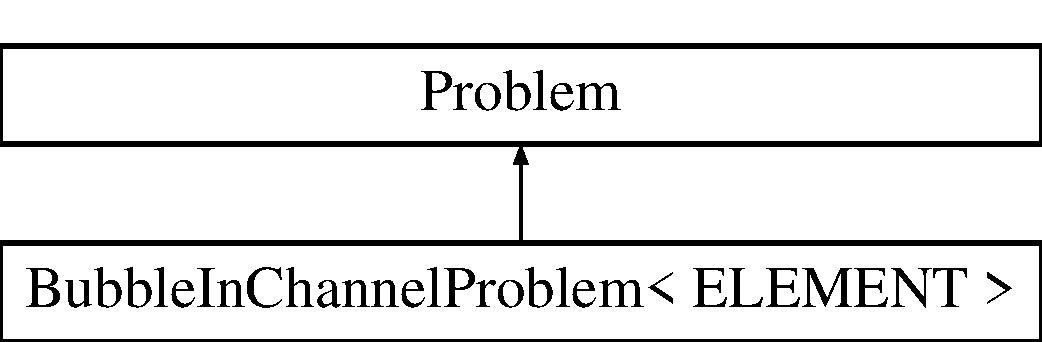
\includegraphics[height=2.000000cm]{classBubbleInChannelProblem}
\end{center}
\end{figure}
\subsection*{Public Member Functions}
\begin{DoxyCompactItemize}
\item 
\hyperlink{classBubbleInChannelProblem_a04bf2f20c65e85228fac381d786bedad}{Bubble\+In\+Channel\+Problem} ()
\begin{DoxyCompactList}\small\item\em Constructor. \end{DoxyCompactList}\item 
\hyperlink{classBubbleInChannelProblem_a7a048a26898571d0f109df2a11f08eb7}{$\sim$\+Bubble\+In\+Channel\+Problem} ()
\begin{DoxyCompactList}\small\item\em Destructor. \end{DoxyCompactList}\item 
void \hyperlink{classBubbleInChannelProblem_aae0753340720453a44622c4dbb8807fb}{actions\+\_\+before\+\_\+adapt} ()
\begin{DoxyCompactList}\small\item\em Actions before adapt\+: Wipe the mesh of free surface elements. \end{DoxyCompactList}\item 
void \hyperlink{classBubbleInChannelProblem_a67d2650bfca3775800784379938a35bc}{actions\+\_\+after\+\_\+adapt} ()
\begin{DoxyCompactList}\small\item\em Actions after adapt\+: Rebuild the mesh of free surface elements. \end{DoxyCompactList}\item 
void \hyperlink{classBubbleInChannelProblem_a566685b0a4f5dda91adbf9c781f9eafb}{actions\+\_\+after\+\_\+newton\+\_\+solve} ()
\begin{DoxyCompactList}\small\item\em Update the after solve (empty) \end{DoxyCompactList}\item 
void \hyperlink{classBubbleInChannelProblem_aef53cd0e961bd899e50806ec39f5a3fd}{actions\+\_\+before\+\_\+newton\+\_\+solve} ()
\begin{DoxyCompactList}\small\item\em Update the problem specs before solve. \end{DoxyCompactList}\item 
void \hyperlink{classBubbleInChannelProblem_a7b3c042477f4ee4e62dd1e00e1a480f8}{complete\+\_\+problem\+\_\+setup} ()
\begin{DoxyCompactList}\small\item\em Set boundary conditions and complete the build of all elements. \end{DoxyCompactList}\item 
void \hyperlink{classBubbleInChannelProblem_a6a68ee06024107d7b3f92059365a06d1}{doc\+\_\+solution} (const std\+::string \&comment=\char`\"{}\char`\"{})
\begin{DoxyCompactList}\small\item\em Doc the solution. \end{DoxyCompactList}\item 
void \hyperlink{classBubbleInChannelProblem_ad400025c03926745e230e5f654c28562}{compute\+\_\+error\+\_\+estimate} (double \&max\+\_\+err, double \&min\+\_\+err)
\begin{DoxyCompactList}\small\item\em Compute the error estimates and assign to elements for plotting. \end{DoxyCompactList}\end{DoxyCompactItemize}
\subsection*{Private Types}
\begin{DoxyCompactItemize}
\item 
enum \{ \newline
\hyperlink{classBubbleInChannelProblem_a5cc2eecaafc178aa80ab1e66bb909fa9a74e672f81a49928bd0d69321acb3f7ea}{Inflow\+\_\+boundary\+\_\+id} =0, 
\hyperlink{classBubbleInChannelProblem_a5cc2eecaafc178aa80ab1e66bb909fa9a52a5fe0a55c757103b9eded639a789fe}{Upper\+\_\+wall\+\_\+boundary\+\_\+id} =1, 
\hyperlink{classBubbleInChannelProblem_a5cc2eecaafc178aa80ab1e66bb909fa9ad7c054a244fe70afadfbae778986e792}{Outflow\+\_\+boundary\+\_\+id} =2, 
\hyperlink{classBubbleInChannelProblem_a5cc2eecaafc178aa80ab1e66bb909fa9a0ad16aa9f84c4a6dadad5eb21c90e3b0}{Bottom\+\_\+wall\+\_\+boundary\+\_\+id} =3, 
\newline
\hyperlink{classBubbleInChannelProblem_a5cc2eecaafc178aa80ab1e66bb909fa9a203cab16fd7ad35c19896ea4eebebf68}{First\+\_\+bubble\+\_\+boundary\+\_\+id} =4, 
\hyperlink{classBubbleInChannelProblem_a5cc2eecaafc178aa80ab1e66bb909fa9a14ffa03e38c0c2bdbfcfe6f190cfae12}{Second\+\_\+bubble\+\_\+boundary\+\_\+id} =5
 \}\begin{DoxyCompactList}\small\item\em Enumeration of mesh boundaries. \end{DoxyCompactList}
\end{DoxyCompactItemize}
\subsection*{Private Member Functions}
\begin{DoxyCompactItemize}
\item 
void \hyperlink{classBubbleInChannelProblem_a9a5a34516352db3153baa52ccb204b62}{create\+\_\+free\+\_\+surface\+\_\+elements} ()
\begin{DoxyCompactList}\small\item\em Create free surface elements. \end{DoxyCompactList}\item 
void \hyperlink{classBubbleInChannelProblem_af660f1a89b325e6da5d040f0abf837b0}{delete\+\_\+free\+\_\+surface\+\_\+elements} ()
\begin{DoxyCompactList}\small\item\em Delete free surface elements. \end{DoxyCompactList}\item 
void \hyperlink{classBubbleInChannelProblem_ae1ab79ef810211e337127878876c0fa6}{create\+\_\+volume\+\_\+constraint\+\_\+elements} ()
\begin{DoxyCompactList}\small\item\em Create elements that impose volume constraint on the bubble. \end{DoxyCompactList}\item 
void \hyperlink{classBubbleInChannelProblem_aecf64bacdf8735910d7dc7d747e1737a}{delete\+\_\+volume\+\_\+constraint\+\_\+elements} ()
\begin{DoxyCompactList}\small\item\em Delete volume constraint elements. \end{DoxyCompactList}\end{DoxyCompactItemize}
\subsection*{Private Attributes}
\begin{DoxyCompactItemize}
\item 
Mesh $\ast$ \hyperlink{classBubbleInChannelProblem_a453d5544b8e936594c1c7f8587e85da2}{Free\+\_\+surface\+\_\+mesh\+\_\+pt}
\begin{DoxyCompactList}\small\item\em Pointers to mesh of free surface elements. \end{DoxyCompactList}\item 
Mesh $\ast$ \hyperlink{classBubbleInChannelProblem_a341644d44c22ff16c9023b614f0c6471}{Volume\+\_\+constraint\+\_\+mesh\+\_\+pt}
\begin{DoxyCompactList}\small\item\em Pointer to mesh containing elements that impose volume constraint. \end{DoxyCompactList}\item 
Refineable\+Solid\+Triangle\+Mesh$<$ E\+L\+E\+M\+E\+NT $>$ $\ast$ \hyperlink{classBubbleInChannelProblem_a1699f6dff44b3d9cb606c7227f5679b7}{Fluid\+\_\+mesh\+\_\+pt}
\begin{DoxyCompactList}\small\item\em Pointer to Fluid\+\_\+mesh. \end{DoxyCompactList}\item 
Vector$<$ Triangle\+Mesh\+Polygon $\ast$ $>$ \hyperlink{classBubbleInChannelProblem_a31c26dd6bdb8071bf80bb7c4b29930d7}{Bubble\+\_\+polygon\+\_\+pt}
\begin{DoxyCompactList}\small\item\em Vector storing pointer to the bubble polygons. \end{DoxyCompactList}\item 
Triangle\+Mesh\+Polygon $\ast$ \hyperlink{classBubbleInChannelProblem_a3a8d8a03e409ce1cfee1f7ce3e1a9434}{Outer\+\_\+boundary\+\_\+polyline\+\_\+pt}
\begin{DoxyCompactList}\small\item\em Triangle mesh polygon for outer boundary. \end{DoxyCompactList}\item 
Data $\ast$ \hyperlink{classBubbleInChannelProblem_a88f2b8e5e56219b8e557d8e78fc5b989}{Bubble\+\_\+pressure\+\_\+data\+\_\+pt}
\begin{DoxyCompactList}\small\item\em Pointer to a global bubble pressure datum. \end{DoxyCompactList}\item 
Volume\+Constraint\+Element $\ast$ \hyperlink{classBubbleInChannelProblem_ac0343258f630d7c0886cca51ba57e80d}{Vol\+\_\+constraint\+\_\+el\+\_\+pt}
\begin{DoxyCompactList}\small\item\em Pointer to element that imposes volume constraint for bubble. \end{DoxyCompactList}\end{DoxyCompactItemize}


\subsection{Detailed Description}
\subsubsection*{template$<$class E\+L\+E\+M\+E\+NT$>$\newline
class Bubble\+In\+Channel\+Problem$<$ E\+L\+E\+M\+E\+N\+T $>$}

Problem class to simulate inviscid bubble propagating along 2D channel. 

Definition at line 428 of file adaptive\+\_\+bubble\+\_\+in\+\_\+channel.\+cc.



\subsection{Member Enumeration Documentation}
\mbox{\Hypertarget{classBubbleInChannelProblem_a5cc2eecaafc178aa80ab1e66bb909fa9}\label{classBubbleInChannelProblem_a5cc2eecaafc178aa80ab1e66bb909fa9}} 
\subsubsection{\texorpdfstring{anonymous enum}{anonymous enum}}
{\footnotesize\ttfamily template$<$class E\+L\+E\+M\+E\+NT$>$ \\
anonymous enum\hspace{0.3cm}{\ttfamily [private]}}



Enumeration of mesh boundaries. 

\begin{DoxyEnumFields}{Enumerator}
\raisebox{\heightof{T}}[0pt][0pt]{\index{Inflow\+\_\+boundary\+\_\+id@{Inflow\+\_\+boundary\+\_\+id}!Bubble\+In\+Channel\+Problem@{Bubble\+In\+Channel\+Problem}}\index{Bubble\+In\+Channel\+Problem@{Bubble\+In\+Channel\+Problem}!Inflow\+\_\+boundary\+\_\+id@{Inflow\+\_\+boundary\+\_\+id}}}\mbox{\Hypertarget{classBubbleInChannelProblem_a5cc2eecaafc178aa80ab1e66bb909fa9a74e672f81a49928bd0d69321acb3f7ea}\label{classBubbleInChannelProblem_a5cc2eecaafc178aa80ab1e66bb909fa9a74e672f81a49928bd0d69321acb3f7ea}} 
Inflow\+\_\+boundary\+\_\+id&\\
\hline

\raisebox{\heightof{T}}[0pt][0pt]{\index{Upper\+\_\+wall\+\_\+boundary\+\_\+id@{Upper\+\_\+wall\+\_\+boundary\+\_\+id}!Bubble\+In\+Channel\+Problem@{Bubble\+In\+Channel\+Problem}}\index{Bubble\+In\+Channel\+Problem@{Bubble\+In\+Channel\+Problem}!Upper\+\_\+wall\+\_\+boundary\+\_\+id@{Upper\+\_\+wall\+\_\+boundary\+\_\+id}}}\mbox{\Hypertarget{classBubbleInChannelProblem_a5cc2eecaafc178aa80ab1e66bb909fa9a52a5fe0a55c757103b9eded639a789fe}\label{classBubbleInChannelProblem_a5cc2eecaafc178aa80ab1e66bb909fa9a52a5fe0a55c757103b9eded639a789fe}} 
Upper\+\_\+wall\+\_\+boundary\+\_\+id&\\
\hline

\raisebox{\heightof{T}}[0pt][0pt]{\index{Outflow\+\_\+boundary\+\_\+id@{Outflow\+\_\+boundary\+\_\+id}!Bubble\+In\+Channel\+Problem@{Bubble\+In\+Channel\+Problem}}\index{Bubble\+In\+Channel\+Problem@{Bubble\+In\+Channel\+Problem}!Outflow\+\_\+boundary\+\_\+id@{Outflow\+\_\+boundary\+\_\+id}}}\mbox{\Hypertarget{classBubbleInChannelProblem_a5cc2eecaafc178aa80ab1e66bb909fa9ad7c054a244fe70afadfbae778986e792}\label{classBubbleInChannelProblem_a5cc2eecaafc178aa80ab1e66bb909fa9ad7c054a244fe70afadfbae778986e792}} 
Outflow\+\_\+boundary\+\_\+id&\\
\hline

\raisebox{\heightof{T}}[0pt][0pt]{\index{Bottom\+\_\+wall\+\_\+boundary\+\_\+id@{Bottom\+\_\+wall\+\_\+boundary\+\_\+id}!Bubble\+In\+Channel\+Problem@{Bubble\+In\+Channel\+Problem}}\index{Bubble\+In\+Channel\+Problem@{Bubble\+In\+Channel\+Problem}!Bottom\+\_\+wall\+\_\+boundary\+\_\+id@{Bottom\+\_\+wall\+\_\+boundary\+\_\+id}}}\mbox{\Hypertarget{classBubbleInChannelProblem_a5cc2eecaafc178aa80ab1e66bb909fa9a0ad16aa9f84c4a6dadad5eb21c90e3b0}\label{classBubbleInChannelProblem_a5cc2eecaafc178aa80ab1e66bb909fa9a0ad16aa9f84c4a6dadad5eb21c90e3b0}} 
Bottom\+\_\+wall\+\_\+boundary\+\_\+id&\\
\hline

\raisebox{\heightof{T}}[0pt][0pt]{\index{First\+\_\+bubble\+\_\+boundary\+\_\+id@{First\+\_\+bubble\+\_\+boundary\+\_\+id}!Bubble\+In\+Channel\+Problem@{Bubble\+In\+Channel\+Problem}}\index{Bubble\+In\+Channel\+Problem@{Bubble\+In\+Channel\+Problem}!First\+\_\+bubble\+\_\+boundary\+\_\+id@{First\+\_\+bubble\+\_\+boundary\+\_\+id}}}\mbox{\Hypertarget{classBubbleInChannelProblem_a5cc2eecaafc178aa80ab1e66bb909fa9a203cab16fd7ad35c19896ea4eebebf68}\label{classBubbleInChannelProblem_a5cc2eecaafc178aa80ab1e66bb909fa9a203cab16fd7ad35c19896ea4eebebf68}} 
First\+\_\+bubble\+\_\+boundary\+\_\+id&\\
\hline

\raisebox{\heightof{T}}[0pt][0pt]{\index{Second\+\_\+bubble\+\_\+boundary\+\_\+id@{Second\+\_\+bubble\+\_\+boundary\+\_\+id}!Bubble\+In\+Channel\+Problem@{Bubble\+In\+Channel\+Problem}}\index{Bubble\+In\+Channel\+Problem@{Bubble\+In\+Channel\+Problem}!Second\+\_\+bubble\+\_\+boundary\+\_\+id@{Second\+\_\+bubble\+\_\+boundary\+\_\+id}}}\mbox{\Hypertarget{classBubbleInChannelProblem_a5cc2eecaafc178aa80ab1e66bb909fa9a14ffa03e38c0c2bdbfcfe6f190cfae12}\label{classBubbleInChannelProblem_a5cc2eecaafc178aa80ab1e66bb909fa9a14ffa03e38c0c2bdbfcfe6f190cfae12}} 
Second\+\_\+bubble\+\_\+boundary\+\_\+id&\\
\hline

\end{DoxyEnumFields}


Definition at line 605 of file adaptive\+\_\+bubble\+\_\+in\+\_\+channel.\+cc.



\subsection{Constructor \& Destructor Documentation}
\mbox{\Hypertarget{classBubbleInChannelProblem_a04bf2f20c65e85228fac381d786bedad}\label{classBubbleInChannelProblem_a04bf2f20c65e85228fac381d786bedad}} 
\index{Bubble\+In\+Channel\+Problem@{Bubble\+In\+Channel\+Problem}!Bubble\+In\+Channel\+Problem@{Bubble\+In\+Channel\+Problem}}
\index{Bubble\+In\+Channel\+Problem@{Bubble\+In\+Channel\+Problem}!Bubble\+In\+Channel\+Problem@{Bubble\+In\+Channel\+Problem}}
\subsubsection{\texorpdfstring{Bubble\+In\+Channel\+Problem()}{BubbleInChannelProblem()}}
{\footnotesize\ttfamily template$<$class E\+L\+E\+M\+E\+NT $>$ \\
\hyperlink{classBubbleInChannelProblem}{Bubble\+In\+Channel\+Problem}$<$ E\+L\+E\+M\+E\+NT $>$\+::\hyperlink{classBubbleInChannelProblem}{Bubble\+In\+Channel\+Problem} (\begin{DoxyParamCaption}{ }\end{DoxyParamCaption})}



Constructor. 



Definition at line 623 of file adaptive\+\_\+bubble\+\_\+in\+\_\+channel.\+cc.



References Problem\+\_\+\+Parameter\+::\+Ca, Problem\+\_\+\+Parameter\+::\+Doc\+\_\+info, Problem\+\_\+\+Parameter\+::\+Length, Problem\+\_\+\+Parameter\+::\+Radius, and Problem\+\_\+\+Parameter\+::\+Volume.

\mbox{\Hypertarget{classBubbleInChannelProblem_a7a048a26898571d0f109df2a11f08eb7}\label{classBubbleInChannelProblem_a7a048a26898571d0f109df2a11f08eb7}} 
\index{Bubble\+In\+Channel\+Problem@{Bubble\+In\+Channel\+Problem}!````~Bubble\+In\+Channel\+Problem@{$\sim$\+Bubble\+In\+Channel\+Problem}}
\index{````~Bubble\+In\+Channel\+Problem@{$\sim$\+Bubble\+In\+Channel\+Problem}!Bubble\+In\+Channel\+Problem@{Bubble\+In\+Channel\+Problem}}
\subsubsection{\texorpdfstring{$\sim$\+Bubble\+In\+Channel\+Problem()}{~BubbleInChannelProblem()}}
{\footnotesize\ttfamily template$<$class E\+L\+E\+M\+E\+NT$>$ \\
\hyperlink{classBubbleInChannelProblem}{Bubble\+In\+Channel\+Problem}$<$ E\+L\+E\+M\+E\+NT $>$\+::$\sim$\hyperlink{classBubbleInChannelProblem}{Bubble\+In\+Channel\+Problem} (\begin{DoxyParamCaption}{ }\end{DoxyParamCaption})\hspace{0.3cm}{\ttfamily [inline]}}



Destructor. 



Definition at line 437 of file adaptive\+\_\+bubble\+\_\+in\+\_\+channel.\+cc.



References Problem\+\_\+\+Parameter\+::\+Constitutive\+\_\+law\+\_\+pt.



\subsection{Member Function Documentation}
\mbox{\Hypertarget{classBubbleInChannelProblem_a67d2650bfca3775800784379938a35bc}\label{classBubbleInChannelProblem_a67d2650bfca3775800784379938a35bc}} 
\index{Bubble\+In\+Channel\+Problem@{Bubble\+In\+Channel\+Problem}!actions\+\_\+after\+\_\+adapt@{actions\+\_\+after\+\_\+adapt}}
\index{actions\+\_\+after\+\_\+adapt@{actions\+\_\+after\+\_\+adapt}!Bubble\+In\+Channel\+Problem@{Bubble\+In\+Channel\+Problem}}
\subsubsection{\texorpdfstring{actions\+\_\+after\+\_\+adapt()}{actions\_after\_adapt()}}
{\footnotesize\ttfamily template$<$class E\+L\+E\+M\+E\+NT$>$ \\
void \hyperlink{classBubbleInChannelProblem}{Bubble\+In\+Channel\+Problem}$<$ E\+L\+E\+M\+E\+NT $>$\+::actions\+\_\+after\+\_\+adapt (\begin{DoxyParamCaption}{ }\end{DoxyParamCaption})\hspace{0.3cm}{\ttfamily [inline]}}



Actions after adapt\+: Rebuild the mesh of free surface elements. 



Definition at line 497 of file adaptive\+\_\+bubble\+\_\+in\+\_\+channel.\+cc.

\mbox{\Hypertarget{classBubbleInChannelProblem_a566685b0a4f5dda91adbf9c781f9eafb}\label{classBubbleInChannelProblem_a566685b0a4f5dda91adbf9c781f9eafb}} 
\index{Bubble\+In\+Channel\+Problem@{Bubble\+In\+Channel\+Problem}!actions\+\_\+after\+\_\+newton\+\_\+solve@{actions\+\_\+after\+\_\+newton\+\_\+solve}}
\index{actions\+\_\+after\+\_\+newton\+\_\+solve@{actions\+\_\+after\+\_\+newton\+\_\+solve}!Bubble\+In\+Channel\+Problem@{Bubble\+In\+Channel\+Problem}}
\subsubsection{\texorpdfstring{actions\+\_\+after\+\_\+newton\+\_\+solve()}{actions\_after\_newton\_solve()}}
{\footnotesize\ttfamily template$<$class E\+L\+E\+M\+E\+NT$>$ \\
void \hyperlink{classBubbleInChannelProblem}{Bubble\+In\+Channel\+Problem}$<$ E\+L\+E\+M\+E\+NT $>$\+::actions\+\_\+after\+\_\+newton\+\_\+solve (\begin{DoxyParamCaption}{ }\end{DoxyParamCaption})\hspace{0.3cm}{\ttfamily [inline]}}



Update the after solve (empty) 



Definition at line 515 of file adaptive\+\_\+bubble\+\_\+in\+\_\+channel.\+cc.

\mbox{\Hypertarget{classBubbleInChannelProblem_aae0753340720453a44622c4dbb8807fb}\label{classBubbleInChannelProblem_aae0753340720453a44622c4dbb8807fb}} 
\index{Bubble\+In\+Channel\+Problem@{Bubble\+In\+Channel\+Problem}!actions\+\_\+before\+\_\+adapt@{actions\+\_\+before\+\_\+adapt}}
\index{actions\+\_\+before\+\_\+adapt@{actions\+\_\+before\+\_\+adapt}!Bubble\+In\+Channel\+Problem@{Bubble\+In\+Channel\+Problem}}
\subsubsection{\texorpdfstring{actions\+\_\+before\+\_\+adapt()}{actions\_before\_adapt()}}
{\footnotesize\ttfamily template$<$class E\+L\+E\+M\+E\+NT$>$ \\
void \hyperlink{classBubbleInChannelProblem}{Bubble\+In\+Channel\+Problem}$<$ E\+L\+E\+M\+E\+NT $>$\+::actions\+\_\+before\+\_\+adapt (\begin{DoxyParamCaption}{ }\end{DoxyParamCaption})\hspace{0.3cm}{\ttfamily [inline]}}



Actions before adapt\+: Wipe the mesh of free surface elements. 



Definition at line 484 of file adaptive\+\_\+bubble\+\_\+in\+\_\+channel.\+cc.

\mbox{\Hypertarget{classBubbleInChannelProblem_aef53cd0e961bd899e50806ec39f5a3fd}\label{classBubbleInChannelProblem_aef53cd0e961bd899e50806ec39f5a3fd}} 
\index{Bubble\+In\+Channel\+Problem@{Bubble\+In\+Channel\+Problem}!actions\+\_\+before\+\_\+newton\+\_\+solve@{actions\+\_\+before\+\_\+newton\+\_\+solve}}
\index{actions\+\_\+before\+\_\+newton\+\_\+solve@{actions\+\_\+before\+\_\+newton\+\_\+solve}!Bubble\+In\+Channel\+Problem@{Bubble\+In\+Channel\+Problem}}
\subsubsection{\texorpdfstring{actions\+\_\+before\+\_\+newton\+\_\+solve()}{actions\_before\_newton\_solve()}}
{\footnotesize\ttfamily template$<$class E\+L\+E\+M\+E\+NT$>$ \\
void \hyperlink{classBubbleInChannelProblem}{Bubble\+In\+Channel\+Problem}$<$ E\+L\+E\+M\+E\+NT $>$\+::actions\+\_\+before\+\_\+newton\+\_\+solve (\begin{DoxyParamCaption}{ }\end{DoxyParamCaption})\hspace{0.3cm}{\ttfamily [inline]}}



Update the problem specs before solve. 



Definition at line 518 of file adaptive\+\_\+bubble\+\_\+in\+\_\+channel.\+cc.

\mbox{\Hypertarget{classBubbleInChannelProblem_a7b3c042477f4ee4e62dd1e00e1a480f8}\label{classBubbleInChannelProblem_a7b3c042477f4ee4e62dd1e00e1a480f8}} 
\index{Bubble\+In\+Channel\+Problem@{Bubble\+In\+Channel\+Problem}!complete\+\_\+problem\+\_\+setup@{complete\+\_\+problem\+\_\+setup}}
\index{complete\+\_\+problem\+\_\+setup@{complete\+\_\+problem\+\_\+setup}!Bubble\+In\+Channel\+Problem@{Bubble\+In\+Channel\+Problem}}
\subsubsection{\texorpdfstring{complete\+\_\+problem\+\_\+setup()}{complete\_problem\_setup()}}
{\footnotesize\ttfamily template$<$class E\+L\+E\+M\+E\+NT $>$ \\
void \hyperlink{classBubbleInChannelProblem}{Bubble\+In\+Channel\+Problem}$<$ E\+L\+E\+M\+E\+NT $>$\+::complete\+\_\+problem\+\_\+setup (\begin{DoxyParamCaption}{ }\end{DoxyParamCaption})}



Set boundary conditions and complete the build of all elements. 



Definition at line 1007 of file adaptive\+\_\+bubble\+\_\+in\+\_\+channel.\+cc.



References Problem\+\_\+\+Parameter\+::\+Constitutive\+\_\+law\+\_\+pt, Problem\+\_\+\+Parameter\+::\+Inflow\+\_\+veloc\+\_\+magnitude, and Problem\+\_\+\+Parameter\+::\+Re.



Referenced by main().

\mbox{\Hypertarget{classBubbleInChannelProblem_ad400025c03926745e230e5f654c28562}\label{classBubbleInChannelProblem_ad400025c03926745e230e5f654c28562}} 
\index{Bubble\+In\+Channel\+Problem@{Bubble\+In\+Channel\+Problem}!compute\+\_\+error\+\_\+estimate@{compute\+\_\+error\+\_\+estimate}}
\index{compute\+\_\+error\+\_\+estimate@{compute\+\_\+error\+\_\+estimate}!Bubble\+In\+Channel\+Problem@{Bubble\+In\+Channel\+Problem}}
\subsubsection{\texorpdfstring{compute\+\_\+error\+\_\+estimate()}{compute\_error\_estimate()}}
{\footnotesize\ttfamily template$<$class E\+L\+E\+M\+E\+NT $>$ \\
void \hyperlink{classBubbleInChannelProblem}{Bubble\+In\+Channel\+Problem}$<$ E\+L\+E\+M\+E\+NT $>$\+::compute\+\_\+error\+\_\+estimate (\begin{DoxyParamCaption}\item[{double \&}]{max\+\_\+err,  }\item[{double \&}]{min\+\_\+err }\end{DoxyParamCaption})}



Compute the error estimates and assign to elements for plotting. 

Compute error estimates and assign to elements for plotting. 

Definition at line 1241 of file adaptive\+\_\+bubble\+\_\+in\+\_\+channel.\+cc.

\mbox{\Hypertarget{classBubbleInChannelProblem_a9a5a34516352db3153baa52ccb204b62}\label{classBubbleInChannelProblem_a9a5a34516352db3153baa52ccb204b62}} 
\index{Bubble\+In\+Channel\+Problem@{Bubble\+In\+Channel\+Problem}!create\+\_\+free\+\_\+surface\+\_\+elements@{create\+\_\+free\+\_\+surface\+\_\+elements}}
\index{create\+\_\+free\+\_\+surface\+\_\+elements@{create\+\_\+free\+\_\+surface\+\_\+elements}!Bubble\+In\+Channel\+Problem@{Bubble\+In\+Channel\+Problem}}
\subsubsection{\texorpdfstring{create\+\_\+free\+\_\+surface\+\_\+elements()}{create\_free\_surface\_elements()}}
{\footnotesize\ttfamily template$<$class E\+L\+E\+M\+E\+NT $>$ \\
void \hyperlink{classBubbleInChannelProblem}{Bubble\+In\+Channel\+Problem}$<$ E\+L\+E\+M\+E\+NT $>$\+::create\+\_\+free\+\_\+surface\+\_\+elements (\begin{DoxyParamCaption}{ }\end{DoxyParamCaption})\hspace{0.3cm}{\ttfamily [private]}}



Create free surface elements. 

Create elements that impose the kinematic and dynamic bcs for the pseudo-\/solid fluid mesh 

Definition at line 904 of file adaptive\+\_\+bubble\+\_\+in\+\_\+channel.\+cc.



References Problem\+\_\+\+Parameter\+::\+Ca.

\mbox{\Hypertarget{classBubbleInChannelProblem_ae1ab79ef810211e337127878876c0fa6}\label{classBubbleInChannelProblem_ae1ab79ef810211e337127878876c0fa6}} 
\index{Bubble\+In\+Channel\+Problem@{Bubble\+In\+Channel\+Problem}!create\+\_\+volume\+\_\+constraint\+\_\+elements@{create\+\_\+volume\+\_\+constraint\+\_\+elements}}
\index{create\+\_\+volume\+\_\+constraint\+\_\+elements@{create\+\_\+volume\+\_\+constraint\+\_\+elements}!Bubble\+In\+Channel\+Problem@{Bubble\+In\+Channel\+Problem}}
\subsubsection{\texorpdfstring{create\+\_\+volume\+\_\+constraint\+\_\+elements()}{create\_volume\_constraint\_elements()}}
{\footnotesize\ttfamily template$<$class E\+L\+E\+M\+E\+NT $>$ \\
void \hyperlink{classBubbleInChannelProblem}{Bubble\+In\+Channel\+Problem}$<$ E\+L\+E\+M\+E\+NT $>$\+::create\+\_\+volume\+\_\+constraint\+\_\+elements (\begin{DoxyParamCaption}{ }\end{DoxyParamCaption})\hspace{0.3cm}{\ttfamily [private]}}



Create elements that impose volume constraint on the bubble. 



Definition at line 962 of file adaptive\+\_\+bubble\+\_\+in\+\_\+channel.\+cc.

\mbox{\Hypertarget{classBubbleInChannelProblem_af660f1a89b325e6da5d040f0abf837b0}\label{classBubbleInChannelProblem_af660f1a89b325e6da5d040f0abf837b0}} 
\index{Bubble\+In\+Channel\+Problem@{Bubble\+In\+Channel\+Problem}!delete\+\_\+free\+\_\+surface\+\_\+elements@{delete\+\_\+free\+\_\+surface\+\_\+elements}}
\index{delete\+\_\+free\+\_\+surface\+\_\+elements@{delete\+\_\+free\+\_\+surface\+\_\+elements}!Bubble\+In\+Channel\+Problem@{Bubble\+In\+Channel\+Problem}}
\subsubsection{\texorpdfstring{delete\+\_\+free\+\_\+surface\+\_\+elements()}{delete\_free\_surface\_elements()}}
{\footnotesize\ttfamily template$<$class E\+L\+E\+M\+E\+NT$>$ \\
void \hyperlink{classBubbleInChannelProblem}{Bubble\+In\+Channel\+Problem}$<$ E\+L\+E\+M\+E\+NT $>$\+::delete\+\_\+free\+\_\+surface\+\_\+elements (\begin{DoxyParamCaption}{ }\end{DoxyParamCaption})\hspace{0.3cm}{\ttfamily [inline]}, {\ttfamily [private]}}



Delete free surface elements. 



Definition at line 543 of file adaptive\+\_\+bubble\+\_\+in\+\_\+channel.\+cc.

\mbox{\Hypertarget{classBubbleInChannelProblem_aecf64bacdf8735910d7dc7d747e1737a}\label{classBubbleInChannelProblem_aecf64bacdf8735910d7dc7d747e1737a}} 
\index{Bubble\+In\+Channel\+Problem@{Bubble\+In\+Channel\+Problem}!delete\+\_\+volume\+\_\+constraint\+\_\+elements@{delete\+\_\+volume\+\_\+constraint\+\_\+elements}}
\index{delete\+\_\+volume\+\_\+constraint\+\_\+elements@{delete\+\_\+volume\+\_\+constraint\+\_\+elements}!Bubble\+In\+Channel\+Problem@{Bubble\+In\+Channel\+Problem}}
\subsubsection{\texorpdfstring{delete\+\_\+volume\+\_\+constraint\+\_\+elements()}{delete\_volume\_constraint\_elements()}}
{\footnotesize\ttfamily template$<$class E\+L\+E\+M\+E\+NT$>$ \\
void \hyperlink{classBubbleInChannelProblem}{Bubble\+In\+Channel\+Problem}$<$ E\+L\+E\+M\+E\+NT $>$\+::delete\+\_\+volume\+\_\+constraint\+\_\+elements (\begin{DoxyParamCaption}{ }\end{DoxyParamCaption})\hspace{0.3cm}{\ttfamily [inline]}, {\ttfamily [private]}}



Delete volume constraint elements. 



Definition at line 565 of file adaptive\+\_\+bubble\+\_\+in\+\_\+channel.\+cc.

\mbox{\Hypertarget{classBubbleInChannelProblem_a6a68ee06024107d7b3f92059365a06d1}\label{classBubbleInChannelProblem_a6a68ee06024107d7b3f92059365a06d1}} 
\index{Bubble\+In\+Channel\+Problem@{Bubble\+In\+Channel\+Problem}!doc\+\_\+solution@{doc\+\_\+solution}}
\index{doc\+\_\+solution@{doc\+\_\+solution}!Bubble\+In\+Channel\+Problem@{Bubble\+In\+Channel\+Problem}}
\subsubsection{\texorpdfstring{doc\+\_\+solution()}{doc\_solution()}}
{\footnotesize\ttfamily template$<$class E\+L\+E\+M\+E\+NT $>$ \\
void \hyperlink{classBubbleInChannelProblem}{Bubble\+In\+Channel\+Problem}$<$ E\+L\+E\+M\+E\+NT $>$\+::doc\+\_\+solution (\begin{DoxyParamCaption}\item[{const std\+::string \&}]{comment = {\ttfamily \char`\"{}\char`\"{}} }\end{DoxyParamCaption})}



Doc the solution. 



Definition at line 1160 of file adaptive\+\_\+bubble\+\_\+in\+\_\+channel.\+cc.



References Problem\+\_\+\+Parameter\+::\+Doc\+\_\+info, Problem\+\_\+\+Parameter\+::\+Norm\+\_\+file, Problem\+\_\+\+Parameter\+::\+Trace\+\_\+file, and Problem\+\_\+\+Parameter\+::\+Volume.



Referenced by main().



\subsection{Member Data Documentation}
\mbox{\Hypertarget{classBubbleInChannelProblem_a31c26dd6bdb8071bf80bb7c4b29930d7}\label{classBubbleInChannelProblem_a31c26dd6bdb8071bf80bb7c4b29930d7}} 
\index{Bubble\+In\+Channel\+Problem@{Bubble\+In\+Channel\+Problem}!Bubble\+\_\+polygon\+\_\+pt@{Bubble\+\_\+polygon\+\_\+pt}}
\index{Bubble\+\_\+polygon\+\_\+pt@{Bubble\+\_\+polygon\+\_\+pt}!Bubble\+In\+Channel\+Problem@{Bubble\+In\+Channel\+Problem}}
\subsubsection{\texorpdfstring{Bubble\+\_\+polygon\+\_\+pt}{Bubble\_polygon\_pt}}
{\footnotesize\ttfamily template$<$class E\+L\+E\+M\+E\+NT$>$ \\
Vector$<$Triangle\+Mesh\+Polygon$\ast$$>$ \hyperlink{classBubbleInChannelProblem}{Bubble\+In\+Channel\+Problem}$<$ E\+L\+E\+M\+E\+NT $>$\+::Bubble\+\_\+polygon\+\_\+pt\hspace{0.3cm}{\ttfamily [private]}}



Vector storing pointer to the bubble polygons. 



Definition at line 593 of file adaptive\+\_\+bubble\+\_\+in\+\_\+channel.\+cc.

\mbox{\Hypertarget{classBubbleInChannelProblem_a88f2b8e5e56219b8e557d8e78fc5b989}\label{classBubbleInChannelProblem_a88f2b8e5e56219b8e557d8e78fc5b989}} 
\index{Bubble\+In\+Channel\+Problem@{Bubble\+In\+Channel\+Problem}!Bubble\+\_\+pressure\+\_\+data\+\_\+pt@{Bubble\+\_\+pressure\+\_\+data\+\_\+pt}}
\index{Bubble\+\_\+pressure\+\_\+data\+\_\+pt@{Bubble\+\_\+pressure\+\_\+data\+\_\+pt}!Bubble\+In\+Channel\+Problem@{Bubble\+In\+Channel\+Problem}}
\subsubsection{\texorpdfstring{Bubble\+\_\+pressure\+\_\+data\+\_\+pt}{Bubble\_pressure\_data\_pt}}
{\footnotesize\ttfamily template$<$class E\+L\+E\+M\+E\+NT$>$ \\
Data$\ast$ \hyperlink{classBubbleInChannelProblem}{Bubble\+In\+Channel\+Problem}$<$ E\+L\+E\+M\+E\+NT $>$\+::Bubble\+\_\+pressure\+\_\+data\+\_\+pt\hspace{0.3cm}{\ttfamily [private]}}



Pointer to a global bubble pressure datum. 



Definition at line 599 of file adaptive\+\_\+bubble\+\_\+in\+\_\+channel.\+cc.

\mbox{\Hypertarget{classBubbleInChannelProblem_a1699f6dff44b3d9cb606c7227f5679b7}\label{classBubbleInChannelProblem_a1699f6dff44b3d9cb606c7227f5679b7}} 
\index{Bubble\+In\+Channel\+Problem@{Bubble\+In\+Channel\+Problem}!Fluid\+\_\+mesh\+\_\+pt@{Fluid\+\_\+mesh\+\_\+pt}}
\index{Fluid\+\_\+mesh\+\_\+pt@{Fluid\+\_\+mesh\+\_\+pt}!Bubble\+In\+Channel\+Problem@{Bubble\+In\+Channel\+Problem}}
\subsubsection{\texorpdfstring{Fluid\+\_\+mesh\+\_\+pt}{Fluid\_mesh\_pt}}
{\footnotesize\ttfamily template$<$class E\+L\+E\+M\+E\+NT$>$ \\
Refineable\+Solid\+Triangle\+Mesh$<$E\+L\+E\+M\+E\+NT$>$$\ast$ \hyperlink{classBubbleInChannelProblem}{Bubble\+In\+Channel\+Problem}$<$ E\+L\+E\+M\+E\+NT $>$\+::Fluid\+\_\+mesh\+\_\+pt\hspace{0.3cm}{\ttfamily [private]}}



Pointer to Fluid\+\_\+mesh. 



Definition at line 590 of file adaptive\+\_\+bubble\+\_\+in\+\_\+channel.\+cc.

\mbox{\Hypertarget{classBubbleInChannelProblem_a453d5544b8e936594c1c7f8587e85da2}\label{classBubbleInChannelProblem_a453d5544b8e936594c1c7f8587e85da2}} 
\index{Bubble\+In\+Channel\+Problem@{Bubble\+In\+Channel\+Problem}!Free\+\_\+surface\+\_\+mesh\+\_\+pt@{Free\+\_\+surface\+\_\+mesh\+\_\+pt}}
\index{Free\+\_\+surface\+\_\+mesh\+\_\+pt@{Free\+\_\+surface\+\_\+mesh\+\_\+pt}!Bubble\+In\+Channel\+Problem@{Bubble\+In\+Channel\+Problem}}
\subsubsection{\texorpdfstring{Free\+\_\+surface\+\_\+mesh\+\_\+pt}{Free\_surface\_mesh\_pt}}
{\footnotesize\ttfamily template$<$class E\+L\+E\+M\+E\+NT$>$ \\
Mesh$\ast$ \hyperlink{classBubbleInChannelProblem}{Bubble\+In\+Channel\+Problem}$<$ E\+L\+E\+M\+E\+NT $>$\+::Free\+\_\+surface\+\_\+mesh\+\_\+pt\hspace{0.3cm}{\ttfamily [private]}}



Pointers to mesh of free surface elements. 



Definition at line 584 of file adaptive\+\_\+bubble\+\_\+in\+\_\+channel.\+cc.

\mbox{\Hypertarget{classBubbleInChannelProblem_a3a8d8a03e409ce1cfee1f7ce3e1a9434}\label{classBubbleInChannelProblem_a3a8d8a03e409ce1cfee1f7ce3e1a9434}} 
\index{Bubble\+In\+Channel\+Problem@{Bubble\+In\+Channel\+Problem}!Outer\+\_\+boundary\+\_\+polyline\+\_\+pt@{Outer\+\_\+boundary\+\_\+polyline\+\_\+pt}}
\index{Outer\+\_\+boundary\+\_\+polyline\+\_\+pt@{Outer\+\_\+boundary\+\_\+polyline\+\_\+pt}!Bubble\+In\+Channel\+Problem@{Bubble\+In\+Channel\+Problem}}
\subsubsection{\texorpdfstring{Outer\+\_\+boundary\+\_\+polyline\+\_\+pt}{Outer\_boundary\_polyline\_pt}}
{\footnotesize\ttfamily template$<$class E\+L\+E\+M\+E\+NT$>$ \\
Triangle\+Mesh\+Polygon$\ast$ \hyperlink{classBubbleInChannelProblem}{Bubble\+In\+Channel\+Problem}$<$ E\+L\+E\+M\+E\+NT $>$\+::Outer\+\_\+boundary\+\_\+polyline\+\_\+pt\hspace{0.3cm}{\ttfamily [private]}}



Triangle mesh polygon for outer boundary. 



Definition at line 596 of file adaptive\+\_\+bubble\+\_\+in\+\_\+channel.\+cc.

\mbox{\Hypertarget{classBubbleInChannelProblem_ac0343258f630d7c0886cca51ba57e80d}\label{classBubbleInChannelProblem_ac0343258f630d7c0886cca51ba57e80d}} 
\index{Bubble\+In\+Channel\+Problem@{Bubble\+In\+Channel\+Problem}!Vol\+\_\+constraint\+\_\+el\+\_\+pt@{Vol\+\_\+constraint\+\_\+el\+\_\+pt}}
\index{Vol\+\_\+constraint\+\_\+el\+\_\+pt@{Vol\+\_\+constraint\+\_\+el\+\_\+pt}!Bubble\+In\+Channel\+Problem@{Bubble\+In\+Channel\+Problem}}
\subsubsection{\texorpdfstring{Vol\+\_\+constraint\+\_\+el\+\_\+pt}{Vol\_constraint\_el\_pt}}
{\footnotesize\ttfamily template$<$class E\+L\+E\+M\+E\+NT$>$ \\
Volume\+Constraint\+Element$\ast$ \hyperlink{classBubbleInChannelProblem}{Bubble\+In\+Channel\+Problem}$<$ E\+L\+E\+M\+E\+NT $>$\+::Vol\+\_\+constraint\+\_\+el\+\_\+pt\hspace{0.3cm}{\ttfamily [private]}}



Pointer to element that imposes volume constraint for bubble. 



Definition at line 602 of file adaptive\+\_\+bubble\+\_\+in\+\_\+channel.\+cc.

\mbox{\Hypertarget{classBubbleInChannelProblem_a341644d44c22ff16c9023b614f0c6471}\label{classBubbleInChannelProblem_a341644d44c22ff16c9023b614f0c6471}} 
\index{Bubble\+In\+Channel\+Problem@{Bubble\+In\+Channel\+Problem}!Volume\+\_\+constraint\+\_\+mesh\+\_\+pt@{Volume\+\_\+constraint\+\_\+mesh\+\_\+pt}}
\index{Volume\+\_\+constraint\+\_\+mesh\+\_\+pt@{Volume\+\_\+constraint\+\_\+mesh\+\_\+pt}!Bubble\+In\+Channel\+Problem@{Bubble\+In\+Channel\+Problem}}
\subsubsection{\texorpdfstring{Volume\+\_\+constraint\+\_\+mesh\+\_\+pt}{Volume\_constraint\_mesh\_pt}}
{\footnotesize\ttfamily template$<$class E\+L\+E\+M\+E\+NT$>$ \\
Mesh$\ast$ \hyperlink{classBubbleInChannelProblem}{Bubble\+In\+Channel\+Problem}$<$ E\+L\+E\+M\+E\+NT $>$\+::Volume\+\_\+constraint\+\_\+mesh\+\_\+pt\hspace{0.3cm}{\ttfamily [private]}}



Pointer to mesh containing elements that impose volume constraint. 



Definition at line 587 of file adaptive\+\_\+bubble\+\_\+in\+\_\+channel.\+cc.



The documentation for this class was generated from the following file\+:\begin{DoxyCompactItemize}
\item 
\hyperlink{adaptive__bubble__in__channel_8cc}{adaptive\+\_\+bubble\+\_\+in\+\_\+channel.\+cc}\end{DoxyCompactItemize}

\hypertarget{classDropInChannelProblem}{}\section{Drop\+In\+Channel\+Problem$<$ E\+L\+E\+M\+E\+NT $>$ Class Template Reference}
\label{classDropInChannelProblem}\index{Drop\+In\+Channel\+Problem$<$ E\+L\+E\+M\+E\+N\+T $>$@{Drop\+In\+Channel\+Problem$<$ E\+L\+E\+M\+E\+N\+T $>$}}


Problem class to simulate viscous drop propagating along 2D channel.  


Inheritance diagram for Drop\+In\+Channel\+Problem$<$ E\+L\+E\+M\+E\+NT $>$\+:\begin{figure}[H]
\begin{center}
\leavevmode
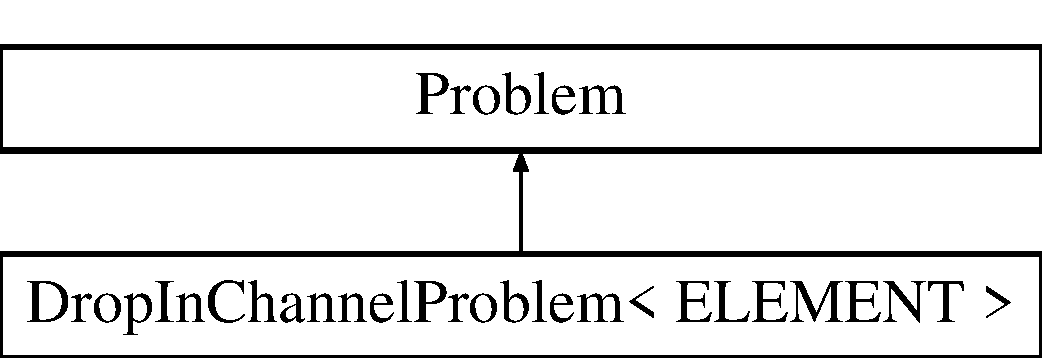
\includegraphics[height=2.000000cm]{classDropInChannelProblem}
\end{center}
\end{figure}
\subsection*{Public Member Functions}
\begin{DoxyCompactItemize}
\item 
\hyperlink{classDropInChannelProblem_aad6e79f5560a5bfcba325f6558afb4ff}{Drop\+In\+Channel\+Problem} ()
\begin{DoxyCompactList}\small\item\em Constructor. \end{DoxyCompactList}\item 
\hyperlink{classDropInChannelProblem_aa311cd8061b915901c8c74617d2e4a37}{$\sim$\+Drop\+In\+Channel\+Problem} ()
\begin{DoxyCompactList}\small\item\em Destructor. \end{DoxyCompactList}\item 
void \hyperlink{classDropInChannelProblem_a4d4ae7fdef14f9838a46cc45278c7920}{actions\+\_\+before\+\_\+adapt} ()
\begin{DoxyCompactList}\small\item\em Actions before adapt\+: Wipe the mesh of free surface elements. \end{DoxyCompactList}\item 
void \hyperlink{classDropInChannelProblem_af5cc96bc60c2fd2386d16eac3ee5f83a}{actions\+\_\+after\+\_\+adapt} ()
\begin{DoxyCompactList}\small\item\em Actions after adapt\+: Rebuild the mesh of free surface elements. \end{DoxyCompactList}\item 
void \hyperlink{classDropInChannelProblem_ab38a14018a4093afe7cc0d9db9f1fc3b}{actions\+\_\+after\+\_\+newton\+\_\+solve} ()
\begin{DoxyCompactList}\small\item\em Update the after solve (empty) \end{DoxyCompactList}\item 
void \hyperlink{classDropInChannelProblem_a0e229343783fd73768dfa0a2672e9ad1}{actions\+\_\+before\+\_\+newton\+\_\+solve} ()
\begin{DoxyCompactList}\small\item\em Update the problem specs before solve. \end{DoxyCompactList}\item 
void \hyperlink{classDropInChannelProblem_a3a868202b34b195a78298b4eaf7d3aff}{complete\+\_\+problem\+\_\+setup} ()
\begin{DoxyCompactList}\small\item\em Set boundary conditions and complete the build of all elements. \end{DoxyCompactList}\item 
void \hyperlink{classDropInChannelProblem_a3bcebc0cd731b75db441f3e1d62296ae}{doc\+\_\+solution} (const std\+::string \&comment=\char`\"{}\char`\"{})
\begin{DoxyCompactList}\small\item\em Doc the solution. \end{DoxyCompactList}\item 
void \hyperlink{classDropInChannelProblem_a49944969eb8dc6892cab3f1a9a2cb382}{compute\+\_\+error\+\_\+estimate} (double \&max\+\_\+err, double \&min\+\_\+err)
\begin{DoxyCompactList}\small\item\em Compute the error estimates and assign to elements for plotting. \end{DoxyCompactList}\item 
void \hyperlink{classDropInChannelProblem_ab8a7491ab12974ccc4cc10bfc0f20675}{remove\+\_\+volume\+\_\+constraint} ()
\begin{DoxyCompactList}\small\item\em Change the boundary conditions to remove the volume constraint. \end{DoxyCompactList}\end{DoxyCompactItemize}
\subsection*{Private Types}
\begin{DoxyCompactItemize}
\item 
enum \{ \newline
\hyperlink{classDropInChannelProblem_a334e4cdb720696ffbc70724caf9b6daba024ca7e6fdbb8bb0dee2984ad4fced0f}{Inflow\+\_\+boundary\+\_\+id} =0, 
\hyperlink{classDropInChannelProblem_a334e4cdb720696ffbc70724caf9b6daba8ce939185dbf37b1b305415c8c73c49c}{Upper\+\_\+wall\+\_\+boundary\+\_\+id} =1, 
\hyperlink{classDropInChannelProblem_a334e4cdb720696ffbc70724caf9b6daba760529dba266f41a831817920ccb1873}{Outflow\+\_\+boundary\+\_\+id} =2, 
\hyperlink{classDropInChannelProblem_a334e4cdb720696ffbc70724caf9b6daba2eb65a21fcbe1b5fe6df3e39edfc3ad7}{Bottom\+\_\+wall\+\_\+boundary\+\_\+id} =3, 
\newline
\hyperlink{classDropInChannelProblem_a334e4cdb720696ffbc70724caf9b6daba7302dcf9298cbc359783e0bc10832a1a}{First\+\_\+drop\+\_\+boundary\+\_\+id} =4, 
\hyperlink{classDropInChannelProblem_a334e4cdb720696ffbc70724caf9b6dababf5c99f82e00ae63a827d4aef8c9d918}{Second\+\_\+drop\+\_\+boundary\+\_\+id} =5
 \}\begin{DoxyCompactList}\small\item\em Enumeration of channel boundaries. \end{DoxyCompactList}
\end{DoxyCompactItemize}
\subsection*{Private Member Functions}
\begin{DoxyCompactItemize}
\item 
void \hyperlink{classDropInChannelProblem_a73b989e3bedbd3630f576b0dba0f724f}{create\+\_\+free\+\_\+surface\+\_\+elements} ()
\begin{DoxyCompactList}\small\item\em Create free surface elements. \end{DoxyCompactList}\item 
void \hyperlink{classDropInChannelProblem_a4463a1b341429f5a2c84a493aabb3a14}{delete\+\_\+free\+\_\+surface\+\_\+elements} ()
\begin{DoxyCompactList}\small\item\em Delete free surface elements. \end{DoxyCompactList}\item 
void \hyperlink{classDropInChannelProblem_a53b96cd50b4e6c9bee294b8fb7dd51bd}{create\+\_\+volume\+\_\+constraint\+\_\+elements} ()
\begin{DoxyCompactList}\small\item\em Create elements that impose volume constraint on the drop. \end{DoxyCompactList}\item 
void \hyperlink{classDropInChannelProblem_aec42cdf762f8b64c064db84df7f40f0a}{delete\+\_\+volume\+\_\+constraint\+\_\+elements} ()
\begin{DoxyCompactList}\small\item\em Delete volume constraint elements. \end{DoxyCompactList}\end{DoxyCompactItemize}
\subsection*{Private Attributes}
\begin{DoxyCompactItemize}
\item 
Mesh $\ast$ \hyperlink{classDropInChannelProblem_a6de0bac4bc483d500aa215a59bbf25bc}{Free\+\_\+surface\+\_\+mesh\+\_\+pt}
\begin{DoxyCompactList}\small\item\em Pointers to mesh of free surface elements. \end{DoxyCompactList}\item 
Mesh $\ast$ \hyperlink{classDropInChannelProblem_ac5f5480fe22c40a175a0b5c0ce39fa05}{Volume\+\_\+constraint\+\_\+mesh\+\_\+pt}
\begin{DoxyCompactList}\small\item\em Pointer to mesh containing elements that impose volume constraint. \end{DoxyCompactList}\item 
Refineable\+Solid\+Triangle\+Mesh$<$ E\+L\+E\+M\+E\+NT $>$ $\ast$ \hyperlink{classDropInChannelProblem_a1f16a75afe9aad09be325d409a4a1b0d}{Fluid\+\_\+mesh\+\_\+pt}
\begin{DoxyCompactList}\small\item\em Pointer to Fluid\+\_\+mesh. \end{DoxyCompactList}\item 
Vector$<$ Triangle\+Mesh\+Polygon $\ast$ $>$ \hyperlink{classDropInChannelProblem_abccd5c5d075bf179150c3d0df25dcea9}{Drop\+\_\+polygon\+\_\+pt}
\begin{DoxyCompactList}\small\item\em Vector storing pointer to the drop polygons. \end{DoxyCompactList}\item 
Triangle\+Mesh\+Polygon $\ast$ \hyperlink{classDropInChannelProblem_aebc1a038a715fd269319b1fb091f0b26}{Outer\+\_\+boundary\+\_\+polyline\+\_\+pt}
\begin{DoxyCompactList}\small\item\em Triangle mesh polygon for outer boundary. \end{DoxyCompactList}\item 
Data $\ast$ \hyperlink{classDropInChannelProblem_ada417f705745bf3e6612f5a9a0a5ef78}{Drop\+\_\+pressure\+\_\+data\+\_\+pt}
\begin{DoxyCompactList}\small\item\em Pointer to a global drop pressure datum. \end{DoxyCompactList}\item 
Volume\+Constraint\+Element $\ast$ \hyperlink{classDropInChannelProblem_ac7476353270d83e26d60f817c371572c}{Vol\+\_\+constraint\+\_\+el\+\_\+pt}
\begin{DoxyCompactList}\small\item\em Pointer to element that imposes volume constraint for drop. \end{DoxyCompactList}\item 
double \hyperlink{classDropInChannelProblem_a0b54287d521735c003d32b71f4f925c3}{Initial\+\_\+value\+\_\+for\+\_\+drop\+\_\+pressure}
\begin{DoxyCompactList}\small\item\em Backed up drop pressure between adaptations. \end{DoxyCompactList}\item 
E\+L\+E\+M\+E\+NT $\ast$ \hyperlink{classDropInChannelProblem_af88997c3a40755063c21e4a95601600a}{Hijacked\+\_\+element\+\_\+pt}
\begin{DoxyCompactList}\small\item\em Pointer to hijacked element. \end{DoxyCompactList}\item 
bool \hyperlink{classDropInChannelProblem_aa555cfd96e802218280acd0165f974dd}{Use\+\_\+volume\+\_\+constraint}
\begin{DoxyCompactList}\small\item\em Bool to indicate if volume constraint is applied (only for steady run) \end{DoxyCompactList}\end{DoxyCompactItemize}


\subsection{Detailed Description}
\subsubsection*{template$<$class E\+L\+E\+M\+E\+NT$>$\newline
class Drop\+In\+Channel\+Problem$<$ E\+L\+E\+M\+E\+N\+T $>$}

Problem class to simulate viscous drop propagating along 2D channel. 

Definition at line 412 of file adaptive\+\_\+drop\+\_\+in\+\_\+channel.\+cc.



\subsection{Member Enumeration Documentation}
\mbox{\Hypertarget{classDropInChannelProblem_a334e4cdb720696ffbc70724caf9b6dab}\label{classDropInChannelProblem_a334e4cdb720696ffbc70724caf9b6dab}} 
\subsubsection{\texorpdfstring{anonymous enum}{anonymous enum}}
{\footnotesize\ttfamily template$<$class E\+L\+E\+M\+E\+NT $>$ \\
anonymous enum\hspace{0.3cm}{\ttfamily [private]}}



Enumeration of channel boundaries. 

\begin{DoxyEnumFields}{Enumerator}
\raisebox{\heightof{T}}[0pt][0pt]{\index{Inflow\+\_\+boundary\+\_\+id@{Inflow\+\_\+boundary\+\_\+id}!Drop\+In\+Channel\+Problem@{Drop\+In\+Channel\+Problem}}\index{Drop\+In\+Channel\+Problem@{Drop\+In\+Channel\+Problem}!Inflow\+\_\+boundary\+\_\+id@{Inflow\+\_\+boundary\+\_\+id}}}\mbox{\Hypertarget{classDropInChannelProblem_a334e4cdb720696ffbc70724caf9b6daba024ca7e6fdbb8bb0dee2984ad4fced0f}\label{classDropInChannelProblem_a334e4cdb720696ffbc70724caf9b6daba024ca7e6fdbb8bb0dee2984ad4fced0f}} 
Inflow\+\_\+boundary\+\_\+id&\\
\hline

\raisebox{\heightof{T}}[0pt][0pt]{\index{Upper\+\_\+wall\+\_\+boundary\+\_\+id@{Upper\+\_\+wall\+\_\+boundary\+\_\+id}!Drop\+In\+Channel\+Problem@{Drop\+In\+Channel\+Problem}}\index{Drop\+In\+Channel\+Problem@{Drop\+In\+Channel\+Problem}!Upper\+\_\+wall\+\_\+boundary\+\_\+id@{Upper\+\_\+wall\+\_\+boundary\+\_\+id}}}\mbox{\Hypertarget{classDropInChannelProblem_a334e4cdb720696ffbc70724caf9b6daba8ce939185dbf37b1b305415c8c73c49c}\label{classDropInChannelProblem_a334e4cdb720696ffbc70724caf9b6daba8ce939185dbf37b1b305415c8c73c49c}} 
Upper\+\_\+wall\+\_\+boundary\+\_\+id&\\
\hline

\raisebox{\heightof{T}}[0pt][0pt]{\index{Outflow\+\_\+boundary\+\_\+id@{Outflow\+\_\+boundary\+\_\+id}!Drop\+In\+Channel\+Problem@{Drop\+In\+Channel\+Problem}}\index{Drop\+In\+Channel\+Problem@{Drop\+In\+Channel\+Problem}!Outflow\+\_\+boundary\+\_\+id@{Outflow\+\_\+boundary\+\_\+id}}}\mbox{\Hypertarget{classDropInChannelProblem_a334e4cdb720696ffbc70724caf9b6daba760529dba266f41a831817920ccb1873}\label{classDropInChannelProblem_a334e4cdb720696ffbc70724caf9b6daba760529dba266f41a831817920ccb1873}} 
Outflow\+\_\+boundary\+\_\+id&\\
\hline

\raisebox{\heightof{T}}[0pt][0pt]{\index{Bottom\+\_\+wall\+\_\+boundary\+\_\+id@{Bottom\+\_\+wall\+\_\+boundary\+\_\+id}!Drop\+In\+Channel\+Problem@{Drop\+In\+Channel\+Problem}}\index{Drop\+In\+Channel\+Problem@{Drop\+In\+Channel\+Problem}!Bottom\+\_\+wall\+\_\+boundary\+\_\+id@{Bottom\+\_\+wall\+\_\+boundary\+\_\+id}}}\mbox{\Hypertarget{classDropInChannelProblem_a334e4cdb720696ffbc70724caf9b6daba2eb65a21fcbe1b5fe6df3e39edfc3ad7}\label{classDropInChannelProblem_a334e4cdb720696ffbc70724caf9b6daba2eb65a21fcbe1b5fe6df3e39edfc3ad7}} 
Bottom\+\_\+wall\+\_\+boundary\+\_\+id&\\
\hline

\raisebox{\heightof{T}}[0pt][0pt]{\index{First\+\_\+drop\+\_\+boundary\+\_\+id@{First\+\_\+drop\+\_\+boundary\+\_\+id}!Drop\+In\+Channel\+Problem@{Drop\+In\+Channel\+Problem}}\index{Drop\+In\+Channel\+Problem@{Drop\+In\+Channel\+Problem}!First\+\_\+drop\+\_\+boundary\+\_\+id@{First\+\_\+drop\+\_\+boundary\+\_\+id}}}\mbox{\Hypertarget{classDropInChannelProblem_a334e4cdb720696ffbc70724caf9b6daba7302dcf9298cbc359783e0bc10832a1a}\label{classDropInChannelProblem_a334e4cdb720696ffbc70724caf9b6daba7302dcf9298cbc359783e0bc10832a1a}} 
First\+\_\+drop\+\_\+boundary\+\_\+id&\\
\hline

\raisebox{\heightof{T}}[0pt][0pt]{\index{Second\+\_\+drop\+\_\+boundary\+\_\+id@{Second\+\_\+drop\+\_\+boundary\+\_\+id}!Drop\+In\+Channel\+Problem@{Drop\+In\+Channel\+Problem}}\index{Drop\+In\+Channel\+Problem@{Drop\+In\+Channel\+Problem}!Second\+\_\+drop\+\_\+boundary\+\_\+id@{Second\+\_\+drop\+\_\+boundary\+\_\+id}}}\mbox{\Hypertarget{classDropInChannelProblem_a334e4cdb720696ffbc70724caf9b6dababf5c99f82e00ae63a827d4aef8c9d918}\label{classDropInChannelProblem_a334e4cdb720696ffbc70724caf9b6dababf5c99f82e00ae63a827d4aef8c9d918}} 
Second\+\_\+drop\+\_\+boundary\+\_\+id&\\
\hline

\end{DoxyEnumFields}


Definition at line 648 of file adaptive\+\_\+drop\+\_\+in\+\_\+channel.\+cc.



\subsection{Constructor \& Destructor Documentation}
\mbox{\Hypertarget{classDropInChannelProblem_aad6e79f5560a5bfcba325f6558afb4ff}\label{classDropInChannelProblem_aad6e79f5560a5bfcba325f6558afb4ff}} 
\index{Drop\+In\+Channel\+Problem@{Drop\+In\+Channel\+Problem}!Drop\+In\+Channel\+Problem@{Drop\+In\+Channel\+Problem}}
\index{Drop\+In\+Channel\+Problem@{Drop\+In\+Channel\+Problem}!Drop\+In\+Channel\+Problem@{Drop\+In\+Channel\+Problem}}
\subsubsection{\texorpdfstring{Drop\+In\+Channel\+Problem()}{DropInChannelProblem()}}
{\footnotesize\ttfamily template$<$class E\+L\+E\+M\+E\+NT $>$ \\
\hyperlink{classDropInChannelProblem}{Drop\+In\+Channel\+Problem}$<$ E\+L\+E\+M\+E\+NT $>$\+::\hyperlink{classDropInChannelProblem}{Drop\+In\+Channel\+Problem} (\begin{DoxyParamCaption}{ }\end{DoxyParamCaption})}



Constructor. 



Definition at line 666 of file adaptive\+\_\+drop\+\_\+in\+\_\+channel.\+cc.



References Problem\+\_\+\+Parameter\+::\+Ca, Problem\+\_\+\+Parameter\+::\+Doc\+\_\+info, Problem\+\_\+\+Parameter\+::\+Length, and Problem\+\_\+\+Parameter\+::\+Radius.

\mbox{\Hypertarget{classDropInChannelProblem_aa311cd8061b915901c8c74617d2e4a37}\label{classDropInChannelProblem_aa311cd8061b915901c8c74617d2e4a37}} 
\index{Drop\+In\+Channel\+Problem@{Drop\+In\+Channel\+Problem}!````~Drop\+In\+Channel\+Problem@{$\sim$\+Drop\+In\+Channel\+Problem}}
\index{````~Drop\+In\+Channel\+Problem@{$\sim$\+Drop\+In\+Channel\+Problem}!Drop\+In\+Channel\+Problem@{Drop\+In\+Channel\+Problem}}
\subsubsection{\texorpdfstring{$\sim$\+Drop\+In\+Channel\+Problem()}{~DropInChannelProblem()}}
{\footnotesize\ttfamily template$<$class E\+L\+E\+M\+E\+NT $>$ \\
\hyperlink{classDropInChannelProblem}{Drop\+In\+Channel\+Problem}$<$ E\+L\+E\+M\+E\+NT $>$\+::$\sim$\hyperlink{classDropInChannelProblem}{Drop\+In\+Channel\+Problem} (\begin{DoxyParamCaption}{ }\end{DoxyParamCaption})\hspace{0.3cm}{\ttfamily [inline]}}



Destructor. 



Definition at line 421 of file adaptive\+\_\+drop\+\_\+in\+\_\+channel.\+cc.



References Problem\+\_\+\+Parameter\+::\+Constitutive\+\_\+law\+\_\+pt.



\subsection{Member Function Documentation}
\mbox{\Hypertarget{classDropInChannelProblem_af5cc96bc60c2fd2386d16eac3ee5f83a}\label{classDropInChannelProblem_af5cc96bc60c2fd2386d16eac3ee5f83a}} 
\index{Drop\+In\+Channel\+Problem@{Drop\+In\+Channel\+Problem}!actions\+\_\+after\+\_\+adapt@{actions\+\_\+after\+\_\+adapt}}
\index{actions\+\_\+after\+\_\+adapt@{actions\+\_\+after\+\_\+adapt}!Drop\+In\+Channel\+Problem@{Drop\+In\+Channel\+Problem}}
\subsubsection{\texorpdfstring{actions\+\_\+after\+\_\+adapt()}{actions\_after\_adapt()}}
{\footnotesize\ttfamily template$<$class E\+L\+E\+M\+E\+NT $>$ \\
void \hyperlink{classDropInChannelProblem}{Drop\+In\+Channel\+Problem}$<$ E\+L\+E\+M\+E\+NT $>$\+::actions\+\_\+after\+\_\+adapt (\begin{DoxyParamCaption}{ }\end{DoxyParamCaption})\hspace{0.3cm}{\ttfamily [inline]}}



Actions after adapt\+: Rebuild the mesh of free surface elements. 



Definition at line 481 of file adaptive\+\_\+drop\+\_\+in\+\_\+channel.\+cc.

\mbox{\Hypertarget{classDropInChannelProblem_ab38a14018a4093afe7cc0d9db9f1fc3b}\label{classDropInChannelProblem_ab38a14018a4093afe7cc0d9db9f1fc3b}} 
\index{Drop\+In\+Channel\+Problem@{Drop\+In\+Channel\+Problem}!actions\+\_\+after\+\_\+newton\+\_\+solve@{actions\+\_\+after\+\_\+newton\+\_\+solve}}
\index{actions\+\_\+after\+\_\+newton\+\_\+solve@{actions\+\_\+after\+\_\+newton\+\_\+solve}!Drop\+In\+Channel\+Problem@{Drop\+In\+Channel\+Problem}}
\subsubsection{\texorpdfstring{actions\+\_\+after\+\_\+newton\+\_\+solve()}{actions\_after\_newton\_solve()}}
{\footnotesize\ttfamily template$<$class E\+L\+E\+M\+E\+NT $>$ \\
void \hyperlink{classDropInChannelProblem}{Drop\+In\+Channel\+Problem}$<$ E\+L\+E\+M\+E\+NT $>$\+::actions\+\_\+after\+\_\+newton\+\_\+solve (\begin{DoxyParamCaption}{ }\end{DoxyParamCaption})\hspace{0.3cm}{\ttfamily [inline]}}



Update the after solve (empty) 



Definition at line 500 of file adaptive\+\_\+drop\+\_\+in\+\_\+channel.\+cc.

\mbox{\Hypertarget{classDropInChannelProblem_a4d4ae7fdef14f9838a46cc45278c7920}\label{classDropInChannelProblem_a4d4ae7fdef14f9838a46cc45278c7920}} 
\index{Drop\+In\+Channel\+Problem@{Drop\+In\+Channel\+Problem}!actions\+\_\+before\+\_\+adapt@{actions\+\_\+before\+\_\+adapt}}
\index{actions\+\_\+before\+\_\+adapt@{actions\+\_\+before\+\_\+adapt}!Drop\+In\+Channel\+Problem@{Drop\+In\+Channel\+Problem}}
\subsubsection{\texorpdfstring{actions\+\_\+before\+\_\+adapt()}{actions\_before\_adapt()}}
{\footnotesize\ttfamily template$<$class E\+L\+E\+M\+E\+NT $>$ \\
void \hyperlink{classDropInChannelProblem}{Drop\+In\+Channel\+Problem}$<$ E\+L\+E\+M\+E\+NT $>$\+::actions\+\_\+before\+\_\+adapt (\begin{DoxyParamCaption}{ }\end{DoxyParamCaption})\hspace{0.3cm}{\ttfamily [inline]}}



Actions before adapt\+: Wipe the mesh of free surface elements. 



Definition at line 468 of file adaptive\+\_\+drop\+\_\+in\+\_\+channel.\+cc.

\mbox{\Hypertarget{classDropInChannelProblem_a0e229343783fd73768dfa0a2672e9ad1}\label{classDropInChannelProblem_a0e229343783fd73768dfa0a2672e9ad1}} 
\index{Drop\+In\+Channel\+Problem@{Drop\+In\+Channel\+Problem}!actions\+\_\+before\+\_\+newton\+\_\+solve@{actions\+\_\+before\+\_\+newton\+\_\+solve}}
\index{actions\+\_\+before\+\_\+newton\+\_\+solve@{actions\+\_\+before\+\_\+newton\+\_\+solve}!Drop\+In\+Channel\+Problem@{Drop\+In\+Channel\+Problem}}
\subsubsection{\texorpdfstring{actions\+\_\+before\+\_\+newton\+\_\+solve()}{actions\_before\_newton\_solve()}}
{\footnotesize\ttfamily template$<$class E\+L\+E\+M\+E\+NT $>$ \\
void \hyperlink{classDropInChannelProblem}{Drop\+In\+Channel\+Problem}$<$ E\+L\+E\+M\+E\+NT $>$\+::actions\+\_\+before\+\_\+newton\+\_\+solve (\begin{DoxyParamCaption}{ }\end{DoxyParamCaption})\hspace{0.3cm}{\ttfamily [inline]}}



Update the problem specs before solve. 



Definition at line 503 of file adaptive\+\_\+drop\+\_\+in\+\_\+channel.\+cc.

\mbox{\Hypertarget{classDropInChannelProblem_a3a868202b34b195a78298b4eaf7d3aff}\label{classDropInChannelProblem_a3a868202b34b195a78298b4eaf7d3aff}} 
\index{Drop\+In\+Channel\+Problem@{Drop\+In\+Channel\+Problem}!complete\+\_\+problem\+\_\+setup@{complete\+\_\+problem\+\_\+setup}}
\index{complete\+\_\+problem\+\_\+setup@{complete\+\_\+problem\+\_\+setup}!Drop\+In\+Channel\+Problem@{Drop\+In\+Channel\+Problem}}
\subsubsection{\texorpdfstring{complete\+\_\+problem\+\_\+setup()}{complete\_problem\_setup()}}
{\footnotesize\ttfamily template$<$class E\+L\+E\+M\+E\+NT $>$ \\
void \hyperlink{classDropInChannelProblem}{Drop\+In\+Channel\+Problem}$<$ E\+L\+E\+M\+E\+NT $>$\+::complete\+\_\+problem\+\_\+setup (\begin{DoxyParamCaption}{ }\end{DoxyParamCaption})}



Set boundary conditions and complete the build of all elements. 



Definition at line 1029 of file adaptive\+\_\+drop\+\_\+in\+\_\+channel.\+cc.



References Problem\+\_\+\+Parameter\+::\+Constitutive\+\_\+law\+\_\+pt, Problem\+\_\+\+Parameter\+::\+Inflow\+\_\+veloc\+\_\+magnitude, Problem\+\_\+\+Parameter\+::\+Re, and Problem\+\_\+\+Parameter\+::\+Viscosity\+\_\+ratio.

\mbox{\Hypertarget{classDropInChannelProblem_a49944969eb8dc6892cab3f1a9a2cb382}\label{classDropInChannelProblem_a49944969eb8dc6892cab3f1a9a2cb382}} 
\index{Drop\+In\+Channel\+Problem@{Drop\+In\+Channel\+Problem}!compute\+\_\+error\+\_\+estimate@{compute\+\_\+error\+\_\+estimate}}
\index{compute\+\_\+error\+\_\+estimate@{compute\+\_\+error\+\_\+estimate}!Drop\+In\+Channel\+Problem@{Drop\+In\+Channel\+Problem}}
\subsubsection{\texorpdfstring{compute\+\_\+error\+\_\+estimate()}{compute\_error\_estimate()}}
{\footnotesize\ttfamily template$<$class E\+L\+E\+M\+E\+NT $>$ \\
void \hyperlink{classDropInChannelProblem}{Drop\+In\+Channel\+Problem}$<$ E\+L\+E\+M\+E\+NT $>$\+::compute\+\_\+error\+\_\+estimate (\begin{DoxyParamCaption}\item[{double \&}]{max\+\_\+err,  }\item[{double \&}]{min\+\_\+err }\end{DoxyParamCaption})}



Compute the error estimates and assign to elements for plotting. 

Compute error estimates and assign to elements for plotting. 

Definition at line 1272 of file adaptive\+\_\+drop\+\_\+in\+\_\+channel.\+cc.

\mbox{\Hypertarget{classDropInChannelProblem_a73b989e3bedbd3630f576b0dba0f724f}\label{classDropInChannelProblem_a73b989e3bedbd3630f576b0dba0f724f}} 
\index{Drop\+In\+Channel\+Problem@{Drop\+In\+Channel\+Problem}!create\+\_\+free\+\_\+surface\+\_\+elements@{create\+\_\+free\+\_\+surface\+\_\+elements}}
\index{create\+\_\+free\+\_\+surface\+\_\+elements@{create\+\_\+free\+\_\+surface\+\_\+elements}!Drop\+In\+Channel\+Problem@{Drop\+In\+Channel\+Problem}}
\subsubsection{\texorpdfstring{create\+\_\+free\+\_\+surface\+\_\+elements()}{create\_free\_surface\_elements()}}
{\footnotesize\ttfamily template$<$class E\+L\+E\+M\+E\+NT $>$ \\
void \hyperlink{classDropInChannelProblem}{Drop\+In\+Channel\+Problem}$<$ E\+L\+E\+M\+E\+NT $>$\+::create\+\_\+free\+\_\+surface\+\_\+elements (\begin{DoxyParamCaption}{ }\end{DoxyParamCaption})\hspace{0.3cm}{\ttfamily [private]}}



Create free surface elements. 

Create elements that impose the kinematic and dynamic bcs for the pseudo-\/solid fluid mesh 

Definition at line 912 of file adaptive\+\_\+drop\+\_\+in\+\_\+channel.\+cc.



References Problem\+\_\+\+Parameter\+::\+Ca.

\mbox{\Hypertarget{classDropInChannelProblem_a53b96cd50b4e6c9bee294b8fb7dd51bd}\label{classDropInChannelProblem_a53b96cd50b4e6c9bee294b8fb7dd51bd}} 
\index{Drop\+In\+Channel\+Problem@{Drop\+In\+Channel\+Problem}!create\+\_\+volume\+\_\+constraint\+\_\+elements@{create\+\_\+volume\+\_\+constraint\+\_\+elements}}
\index{create\+\_\+volume\+\_\+constraint\+\_\+elements@{create\+\_\+volume\+\_\+constraint\+\_\+elements}!Drop\+In\+Channel\+Problem@{Drop\+In\+Channel\+Problem}}
\subsubsection{\texorpdfstring{create\+\_\+volume\+\_\+constraint\+\_\+elements()}{create\_volume\_constraint\_elements()}}
{\footnotesize\ttfamily template$<$class E\+L\+E\+M\+E\+NT $>$ \\
void \hyperlink{classDropInChannelProblem}{Drop\+In\+Channel\+Problem}$<$ E\+L\+E\+M\+E\+NT $>$\+::create\+\_\+volume\+\_\+constraint\+\_\+elements (\begin{DoxyParamCaption}{ }\end{DoxyParamCaption})\hspace{0.3cm}{\ttfamily [private]}}



Create elements that impose volume constraint on the drop. 



Definition at line 960 of file adaptive\+\_\+drop\+\_\+in\+\_\+channel.\+cc.



References Problem\+\_\+\+Parameter\+::\+Volume.

\mbox{\Hypertarget{classDropInChannelProblem_a4463a1b341429f5a2c84a493aabb3a14}\label{classDropInChannelProblem_a4463a1b341429f5a2c84a493aabb3a14}} 
\index{Drop\+In\+Channel\+Problem@{Drop\+In\+Channel\+Problem}!delete\+\_\+free\+\_\+surface\+\_\+elements@{delete\+\_\+free\+\_\+surface\+\_\+elements}}
\index{delete\+\_\+free\+\_\+surface\+\_\+elements@{delete\+\_\+free\+\_\+surface\+\_\+elements}!Drop\+In\+Channel\+Problem@{Drop\+In\+Channel\+Problem}}
\subsubsection{\texorpdfstring{delete\+\_\+free\+\_\+surface\+\_\+elements()}{delete\_free\_surface\_elements()}}
{\footnotesize\ttfamily template$<$class E\+L\+E\+M\+E\+NT $>$ \\
void \hyperlink{classDropInChannelProblem}{Drop\+In\+Channel\+Problem}$<$ E\+L\+E\+M\+E\+NT $>$\+::delete\+\_\+free\+\_\+surface\+\_\+elements (\begin{DoxyParamCaption}{ }\end{DoxyParamCaption})\hspace{0.3cm}{\ttfamily [inline]}, {\ttfamily [private]}}



Delete free surface elements. 



Definition at line 565 of file adaptive\+\_\+drop\+\_\+in\+\_\+channel.\+cc.

\mbox{\Hypertarget{classDropInChannelProblem_aec42cdf762f8b64c064db84df7f40f0a}\label{classDropInChannelProblem_aec42cdf762f8b64c064db84df7f40f0a}} 
\index{Drop\+In\+Channel\+Problem@{Drop\+In\+Channel\+Problem}!delete\+\_\+volume\+\_\+constraint\+\_\+elements@{delete\+\_\+volume\+\_\+constraint\+\_\+elements}}
\index{delete\+\_\+volume\+\_\+constraint\+\_\+elements@{delete\+\_\+volume\+\_\+constraint\+\_\+elements}!Drop\+In\+Channel\+Problem@{Drop\+In\+Channel\+Problem}}
\subsubsection{\texorpdfstring{delete\+\_\+volume\+\_\+constraint\+\_\+elements()}{delete\_volume\_constraint\_elements()}}
{\footnotesize\ttfamily template$<$class E\+L\+E\+M\+E\+NT $>$ \\
void \hyperlink{classDropInChannelProblem}{Drop\+In\+Channel\+Problem}$<$ E\+L\+E\+M\+E\+NT $>$\+::delete\+\_\+volume\+\_\+constraint\+\_\+elements (\begin{DoxyParamCaption}{ }\end{DoxyParamCaption})\hspace{0.3cm}{\ttfamily [inline]}, {\ttfamily [private]}}



Delete volume constraint elements. 



Definition at line 589 of file adaptive\+\_\+drop\+\_\+in\+\_\+channel.\+cc.

\mbox{\Hypertarget{classDropInChannelProblem_a3bcebc0cd731b75db441f3e1d62296ae}\label{classDropInChannelProblem_a3bcebc0cd731b75db441f3e1d62296ae}} 
\index{Drop\+In\+Channel\+Problem@{Drop\+In\+Channel\+Problem}!doc\+\_\+solution@{doc\+\_\+solution}}
\index{doc\+\_\+solution@{doc\+\_\+solution}!Drop\+In\+Channel\+Problem@{Drop\+In\+Channel\+Problem}}
\subsubsection{\texorpdfstring{doc\+\_\+solution()}{doc\_solution()}}
{\footnotesize\ttfamily template$<$class E\+L\+E\+M\+E\+NT $>$ \\
void \hyperlink{classDropInChannelProblem}{Drop\+In\+Channel\+Problem}$<$ E\+L\+E\+M\+E\+NT $>$\+::doc\+\_\+solution (\begin{DoxyParamCaption}\item[{const std\+::string \&}]{comment = {\ttfamily \char`\"{}\char`\"{}} }\end{DoxyParamCaption})}



Doc the solution. 



Definition at line 1195 of file adaptive\+\_\+drop\+\_\+in\+\_\+channel.\+cc.



References Problem\+\_\+\+Parameter\+::\+Doc\+\_\+info, Problem\+\_\+\+Parameter\+::\+Norm\+\_\+file, and Problem\+\_\+\+Parameter\+::\+Trace\+\_\+file.

\mbox{\Hypertarget{classDropInChannelProblem_ab8a7491ab12974ccc4cc10bfc0f20675}\label{classDropInChannelProblem_ab8a7491ab12974ccc4cc10bfc0f20675}} 
\index{Drop\+In\+Channel\+Problem@{Drop\+In\+Channel\+Problem}!remove\+\_\+volume\+\_\+constraint@{remove\+\_\+volume\+\_\+constraint}}
\index{remove\+\_\+volume\+\_\+constraint@{remove\+\_\+volume\+\_\+constraint}!Drop\+In\+Channel\+Problem@{Drop\+In\+Channel\+Problem}}
\subsubsection{\texorpdfstring{remove\+\_\+volume\+\_\+constraint()}{remove\_volume\_constraint()}}
{\footnotesize\ttfamily template$<$class E\+L\+E\+M\+E\+NT $>$ \\
void \hyperlink{classDropInChannelProblem}{Drop\+In\+Channel\+Problem}$<$ E\+L\+E\+M\+E\+NT $>$\+::remove\+\_\+volume\+\_\+constraint (\begin{DoxyParamCaption}{ }\end{DoxyParamCaption})\hspace{0.3cm}{\ttfamily [inline]}}



Change the boundary conditions to remove the volume constraint. 



Definition at line 523 of file adaptive\+\_\+drop\+\_\+in\+\_\+channel.\+cc.



\subsection{Member Data Documentation}
\mbox{\Hypertarget{classDropInChannelProblem_abccd5c5d075bf179150c3d0df25dcea9}\label{classDropInChannelProblem_abccd5c5d075bf179150c3d0df25dcea9}} 
\index{Drop\+In\+Channel\+Problem@{Drop\+In\+Channel\+Problem}!Drop\+\_\+polygon\+\_\+pt@{Drop\+\_\+polygon\+\_\+pt}}
\index{Drop\+\_\+polygon\+\_\+pt@{Drop\+\_\+polygon\+\_\+pt}!Drop\+In\+Channel\+Problem@{Drop\+In\+Channel\+Problem}}
\subsubsection{\texorpdfstring{Drop\+\_\+polygon\+\_\+pt}{Drop\_polygon\_pt}}
{\footnotesize\ttfamily template$<$class E\+L\+E\+M\+E\+NT $>$ \\
Vector$<$Triangle\+Mesh\+Polygon$\ast$$>$ \hyperlink{classDropInChannelProblem}{Drop\+In\+Channel\+Problem}$<$ E\+L\+E\+M\+E\+NT $>$\+::Drop\+\_\+polygon\+\_\+pt\hspace{0.3cm}{\ttfamily [private]}}



Vector storing pointer to the drop polygons. 



Definition at line 627 of file adaptive\+\_\+drop\+\_\+in\+\_\+channel.\+cc.

\mbox{\Hypertarget{classDropInChannelProblem_ada417f705745bf3e6612f5a9a0a5ef78}\label{classDropInChannelProblem_ada417f705745bf3e6612f5a9a0a5ef78}} 
\index{Drop\+In\+Channel\+Problem@{Drop\+In\+Channel\+Problem}!Drop\+\_\+pressure\+\_\+data\+\_\+pt@{Drop\+\_\+pressure\+\_\+data\+\_\+pt}}
\index{Drop\+\_\+pressure\+\_\+data\+\_\+pt@{Drop\+\_\+pressure\+\_\+data\+\_\+pt}!Drop\+In\+Channel\+Problem@{Drop\+In\+Channel\+Problem}}
\subsubsection{\texorpdfstring{Drop\+\_\+pressure\+\_\+data\+\_\+pt}{Drop\_pressure\_data\_pt}}
{\footnotesize\ttfamily template$<$class E\+L\+E\+M\+E\+NT $>$ \\
Data$\ast$ \hyperlink{classDropInChannelProblem}{Drop\+In\+Channel\+Problem}$<$ E\+L\+E\+M\+E\+NT $>$\+::Drop\+\_\+pressure\+\_\+data\+\_\+pt\hspace{0.3cm}{\ttfamily [private]}}



Pointer to a global drop pressure datum. 



Definition at line 633 of file adaptive\+\_\+drop\+\_\+in\+\_\+channel.\+cc.

\mbox{\Hypertarget{classDropInChannelProblem_a1f16a75afe9aad09be325d409a4a1b0d}\label{classDropInChannelProblem_a1f16a75afe9aad09be325d409a4a1b0d}} 
\index{Drop\+In\+Channel\+Problem@{Drop\+In\+Channel\+Problem}!Fluid\+\_\+mesh\+\_\+pt@{Fluid\+\_\+mesh\+\_\+pt}}
\index{Fluid\+\_\+mesh\+\_\+pt@{Fluid\+\_\+mesh\+\_\+pt}!Drop\+In\+Channel\+Problem@{Drop\+In\+Channel\+Problem}}
\subsubsection{\texorpdfstring{Fluid\+\_\+mesh\+\_\+pt}{Fluid\_mesh\_pt}}
{\footnotesize\ttfamily template$<$class E\+L\+E\+M\+E\+NT $>$ \\
Refineable\+Solid\+Triangle\+Mesh$<$E\+L\+E\+M\+E\+NT$>$$\ast$ \hyperlink{classDropInChannelProblem}{Drop\+In\+Channel\+Problem}$<$ E\+L\+E\+M\+E\+NT $>$\+::Fluid\+\_\+mesh\+\_\+pt\hspace{0.3cm}{\ttfamily [private]}}



Pointer to Fluid\+\_\+mesh. 



Definition at line 624 of file adaptive\+\_\+drop\+\_\+in\+\_\+channel.\+cc.

\mbox{\Hypertarget{classDropInChannelProblem_a6de0bac4bc483d500aa215a59bbf25bc}\label{classDropInChannelProblem_a6de0bac4bc483d500aa215a59bbf25bc}} 
\index{Drop\+In\+Channel\+Problem@{Drop\+In\+Channel\+Problem}!Free\+\_\+surface\+\_\+mesh\+\_\+pt@{Free\+\_\+surface\+\_\+mesh\+\_\+pt}}
\index{Free\+\_\+surface\+\_\+mesh\+\_\+pt@{Free\+\_\+surface\+\_\+mesh\+\_\+pt}!Drop\+In\+Channel\+Problem@{Drop\+In\+Channel\+Problem}}
\subsubsection{\texorpdfstring{Free\+\_\+surface\+\_\+mesh\+\_\+pt}{Free\_surface\_mesh\_pt}}
{\footnotesize\ttfamily template$<$class E\+L\+E\+M\+E\+NT $>$ \\
Mesh$\ast$ \hyperlink{classDropInChannelProblem}{Drop\+In\+Channel\+Problem}$<$ E\+L\+E\+M\+E\+NT $>$\+::Free\+\_\+surface\+\_\+mesh\+\_\+pt\hspace{0.3cm}{\ttfamily [private]}}



Pointers to mesh of free surface elements. 



Definition at line 618 of file adaptive\+\_\+drop\+\_\+in\+\_\+channel.\+cc.

\mbox{\Hypertarget{classDropInChannelProblem_af88997c3a40755063c21e4a95601600a}\label{classDropInChannelProblem_af88997c3a40755063c21e4a95601600a}} 
\index{Drop\+In\+Channel\+Problem@{Drop\+In\+Channel\+Problem}!Hijacked\+\_\+element\+\_\+pt@{Hijacked\+\_\+element\+\_\+pt}}
\index{Hijacked\+\_\+element\+\_\+pt@{Hijacked\+\_\+element\+\_\+pt}!Drop\+In\+Channel\+Problem@{Drop\+In\+Channel\+Problem}}
\subsubsection{\texorpdfstring{Hijacked\+\_\+element\+\_\+pt}{Hijacked\_element\_pt}}
{\footnotesize\ttfamily template$<$class E\+L\+E\+M\+E\+NT $>$ \\
E\+L\+E\+M\+E\+NT$\ast$ \hyperlink{classDropInChannelProblem}{Drop\+In\+Channel\+Problem}$<$ E\+L\+E\+M\+E\+NT $>$\+::Hijacked\+\_\+element\+\_\+pt\hspace{0.3cm}{\ttfamily [private]}}



Pointer to hijacked element. 



Definition at line 642 of file adaptive\+\_\+drop\+\_\+in\+\_\+channel.\+cc.

\mbox{\Hypertarget{classDropInChannelProblem_a0b54287d521735c003d32b71f4f925c3}\label{classDropInChannelProblem_a0b54287d521735c003d32b71f4f925c3}} 
\index{Drop\+In\+Channel\+Problem@{Drop\+In\+Channel\+Problem}!Initial\+\_\+value\+\_\+for\+\_\+drop\+\_\+pressure@{Initial\+\_\+value\+\_\+for\+\_\+drop\+\_\+pressure}}
\index{Initial\+\_\+value\+\_\+for\+\_\+drop\+\_\+pressure@{Initial\+\_\+value\+\_\+for\+\_\+drop\+\_\+pressure}!Drop\+In\+Channel\+Problem@{Drop\+In\+Channel\+Problem}}
\subsubsection{\texorpdfstring{Initial\+\_\+value\+\_\+for\+\_\+drop\+\_\+pressure}{Initial\_value\_for\_drop\_pressure}}
{\footnotesize\ttfamily template$<$class E\+L\+E\+M\+E\+NT $>$ \\
double \hyperlink{classDropInChannelProblem}{Drop\+In\+Channel\+Problem}$<$ E\+L\+E\+M\+E\+NT $>$\+::Initial\+\_\+value\+\_\+for\+\_\+drop\+\_\+pressure\hspace{0.3cm}{\ttfamily [private]}}



Backed up drop pressure between adaptations. 



Definition at line 639 of file adaptive\+\_\+drop\+\_\+in\+\_\+channel.\+cc.

\mbox{\Hypertarget{classDropInChannelProblem_aebc1a038a715fd269319b1fb091f0b26}\label{classDropInChannelProblem_aebc1a038a715fd269319b1fb091f0b26}} 
\index{Drop\+In\+Channel\+Problem@{Drop\+In\+Channel\+Problem}!Outer\+\_\+boundary\+\_\+polyline\+\_\+pt@{Outer\+\_\+boundary\+\_\+polyline\+\_\+pt}}
\index{Outer\+\_\+boundary\+\_\+polyline\+\_\+pt@{Outer\+\_\+boundary\+\_\+polyline\+\_\+pt}!Drop\+In\+Channel\+Problem@{Drop\+In\+Channel\+Problem}}
\subsubsection{\texorpdfstring{Outer\+\_\+boundary\+\_\+polyline\+\_\+pt}{Outer\_boundary\_polyline\_pt}}
{\footnotesize\ttfamily template$<$class E\+L\+E\+M\+E\+NT $>$ \\
Triangle\+Mesh\+Polygon$\ast$ \hyperlink{classDropInChannelProblem}{Drop\+In\+Channel\+Problem}$<$ E\+L\+E\+M\+E\+NT $>$\+::Outer\+\_\+boundary\+\_\+polyline\+\_\+pt\hspace{0.3cm}{\ttfamily [private]}}



Triangle mesh polygon for outer boundary. 



Definition at line 630 of file adaptive\+\_\+drop\+\_\+in\+\_\+channel.\+cc.

\mbox{\Hypertarget{classDropInChannelProblem_aa555cfd96e802218280acd0165f974dd}\label{classDropInChannelProblem_aa555cfd96e802218280acd0165f974dd}} 
\index{Drop\+In\+Channel\+Problem@{Drop\+In\+Channel\+Problem}!Use\+\_\+volume\+\_\+constraint@{Use\+\_\+volume\+\_\+constraint}}
\index{Use\+\_\+volume\+\_\+constraint@{Use\+\_\+volume\+\_\+constraint}!Drop\+In\+Channel\+Problem@{Drop\+In\+Channel\+Problem}}
\subsubsection{\texorpdfstring{Use\+\_\+volume\+\_\+constraint}{Use\_volume\_constraint}}
{\footnotesize\ttfamily template$<$class E\+L\+E\+M\+E\+NT $>$ \\
bool \hyperlink{classDropInChannelProblem}{Drop\+In\+Channel\+Problem}$<$ E\+L\+E\+M\+E\+NT $>$\+::Use\+\_\+volume\+\_\+constraint\hspace{0.3cm}{\ttfamily [private]}}



Bool to indicate if volume constraint is applied (only for steady run) 



Definition at line 645 of file adaptive\+\_\+drop\+\_\+in\+\_\+channel.\+cc.

\mbox{\Hypertarget{classDropInChannelProblem_ac7476353270d83e26d60f817c371572c}\label{classDropInChannelProblem_ac7476353270d83e26d60f817c371572c}} 
\index{Drop\+In\+Channel\+Problem@{Drop\+In\+Channel\+Problem}!Vol\+\_\+constraint\+\_\+el\+\_\+pt@{Vol\+\_\+constraint\+\_\+el\+\_\+pt}}
\index{Vol\+\_\+constraint\+\_\+el\+\_\+pt@{Vol\+\_\+constraint\+\_\+el\+\_\+pt}!Drop\+In\+Channel\+Problem@{Drop\+In\+Channel\+Problem}}
\subsubsection{\texorpdfstring{Vol\+\_\+constraint\+\_\+el\+\_\+pt}{Vol\_constraint\_el\_pt}}
{\footnotesize\ttfamily template$<$class E\+L\+E\+M\+E\+NT $>$ \\
Volume\+Constraint\+Element$\ast$ \hyperlink{classDropInChannelProblem}{Drop\+In\+Channel\+Problem}$<$ E\+L\+E\+M\+E\+NT $>$\+::Vol\+\_\+constraint\+\_\+el\+\_\+pt\hspace{0.3cm}{\ttfamily [private]}}



Pointer to element that imposes volume constraint for drop. 



Definition at line 636 of file adaptive\+\_\+drop\+\_\+in\+\_\+channel.\+cc.

\mbox{\Hypertarget{classDropInChannelProblem_ac5f5480fe22c40a175a0b5c0ce39fa05}\label{classDropInChannelProblem_ac5f5480fe22c40a175a0b5c0ce39fa05}} 
\index{Drop\+In\+Channel\+Problem@{Drop\+In\+Channel\+Problem}!Volume\+\_\+constraint\+\_\+mesh\+\_\+pt@{Volume\+\_\+constraint\+\_\+mesh\+\_\+pt}}
\index{Volume\+\_\+constraint\+\_\+mesh\+\_\+pt@{Volume\+\_\+constraint\+\_\+mesh\+\_\+pt}!Drop\+In\+Channel\+Problem@{Drop\+In\+Channel\+Problem}}
\subsubsection{\texorpdfstring{Volume\+\_\+constraint\+\_\+mesh\+\_\+pt}{Volume\_constraint\_mesh\_pt}}
{\footnotesize\ttfamily template$<$class E\+L\+E\+M\+E\+NT $>$ \\
Mesh$\ast$ \hyperlink{classDropInChannelProblem}{Drop\+In\+Channel\+Problem}$<$ E\+L\+E\+M\+E\+NT $>$\+::Volume\+\_\+constraint\+\_\+mesh\+\_\+pt\hspace{0.3cm}{\ttfamily [private]}}



Pointer to mesh containing elements that impose volume constraint. 



Definition at line 621 of file adaptive\+\_\+drop\+\_\+in\+\_\+channel.\+cc.



The documentation for this class was generated from the following file\+:\begin{DoxyCompactItemize}
\item 
\hyperlink{adaptive__drop__in__channel_8cc}{adaptive\+\_\+drop\+\_\+in\+\_\+channel.\+cc}\end{DoxyCompactItemize}

\hypertarget{classoomph_1_1FaceGeometry_3_01FaceGeometry_3_01MyCrouzeixRaviartElement_01_4_01_4}{}\section{oomph\+:\+:Face\+Geometry$<$ Face\+Geometry$<$ My\+Crouzeix\+Raviart\+Element $>$ $>$ Class Template Reference}
\label{classoomph_1_1FaceGeometry_3_01FaceGeometry_3_01MyCrouzeixRaviartElement_01_4_01_4}\index{oomph\+::\+Face\+Geometry$<$ Face\+Geometry$<$ My\+Crouzeix\+Raviart\+Element $>$ $>$@{oomph\+::\+Face\+Geometry$<$ Face\+Geometry$<$ My\+Crouzeix\+Raviart\+Element $>$ $>$}}
Inheritance diagram for oomph\+:\+:Face\+Geometry$<$ Face\+Geometry$<$ My\+Crouzeix\+Raviart\+Element $>$ $>$\+:\begin{figure}[H]
\begin{center}
\leavevmode
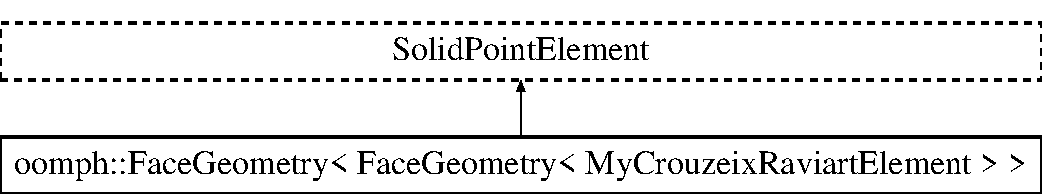
\includegraphics[height=2.000000cm]{classoomph_1_1FaceGeometry_3_01FaceGeometry_3_01MyCrouzeixRaviartElement_01_4_01_4}
\end{center}
\end{figure}
\subsection*{Public Member Functions}
\begin{DoxyCompactItemize}
\item 
\hyperlink{classoomph_1_1FaceGeometry_3_01FaceGeometry_3_01MyCrouzeixRaviartElement_01_4_01_4_ace1479da1535c271d7dc671dacbbdcca}{Face\+Geometry} ()
\end{DoxyCompactItemize}


\subsection{Detailed Description}
\subsubsection*{template$<$$>$\newline
class oomph\+::\+Face\+Geometry$<$ Face\+Geometry$<$ My\+Crouzeix\+Raviart\+Element $>$ $>$}

Face geometry of Face geometry for element is the same as that for the underlying wrapped element 

Definition at line 341 of file adaptive\+\_\+drop\+\_\+in\+\_\+channel.\+cc.



\subsection{Constructor \& Destructor Documentation}
\mbox{\Hypertarget{classoomph_1_1FaceGeometry_3_01FaceGeometry_3_01MyCrouzeixRaviartElement_01_4_01_4_ace1479da1535c271d7dc671dacbbdcca}\label{classoomph_1_1FaceGeometry_3_01FaceGeometry_3_01MyCrouzeixRaviartElement_01_4_01_4_ace1479da1535c271d7dc671dacbbdcca}} 
\index{oomph\+::\+Face\+Geometry$<$ Face\+Geometry$<$ My\+Crouzeix\+Raviart\+Element $>$ $>$@{oomph\+::\+Face\+Geometry$<$ Face\+Geometry$<$ My\+Crouzeix\+Raviart\+Element $>$ $>$}!Face\+Geometry@{Face\+Geometry}}
\index{Face\+Geometry@{Face\+Geometry}!oomph\+::\+Face\+Geometry$<$ Face\+Geometry$<$ My\+Crouzeix\+Raviart\+Element $>$ $>$@{oomph\+::\+Face\+Geometry$<$ Face\+Geometry$<$ My\+Crouzeix\+Raviart\+Element $>$ $>$}}
\subsubsection{\texorpdfstring{Face\+Geometry()}{FaceGeometry()}}
{\footnotesize\ttfamily oomph\+::\+Face\+Geometry$<$ Face\+Geometry$<$ \hyperlink{classoomph_1_1MyCrouzeixRaviartElement}{My\+Crouzeix\+Raviart\+Element} $>$ $>$\+::Face\+Geometry (\begin{DoxyParamCaption}{ }\end{DoxyParamCaption})\hspace{0.3cm}{\ttfamily [inline]}}



Definition at line 345 of file adaptive\+\_\+drop\+\_\+in\+\_\+channel.\+cc.



References Problem\+\_\+\+Parameter\+::\+Ca, Problem\+\_\+\+Parameter\+::\+Doc\+\_\+info, Problem\+\_\+\+Parameter\+::\+Nu, Problem\+\_\+\+Parameter\+::\+Radius, and Problem\+\_\+\+Parameter\+::\+Re.



The documentation for this class was generated from the following file\+:\begin{DoxyCompactItemize}
\item 
\hyperlink{adaptive__drop__in__channel_8cc}{adaptive\+\_\+drop\+\_\+in\+\_\+channel.\+cc}\end{DoxyCompactItemize}

\hypertarget{classoomph_1_1FaceGeometry_3_01FaceGeometry_3_01MyTaylorHoodElement_01_4_01_4}{}\section{oomph\+:\+:Face\+Geometry$<$ Face\+Geometry$<$ My\+Taylor\+Hood\+Element $>$ $>$ Class Template Reference}
\label{classoomph_1_1FaceGeometry_3_01FaceGeometry_3_01MyTaylorHoodElement_01_4_01_4}\index{oomph\+::\+Face\+Geometry$<$ Face\+Geometry$<$ My\+Taylor\+Hood\+Element $>$ $>$@{oomph\+::\+Face\+Geometry$<$ Face\+Geometry$<$ My\+Taylor\+Hood\+Element $>$ $>$}}


{\ttfamily \#include $<$my\+\_\+taylor\+\_\+hood\+\_\+elements.\+h$>$}

Inheritance diagram for oomph\+:\+:Face\+Geometry$<$ Face\+Geometry$<$ My\+Taylor\+Hood\+Element $>$ $>$\+:\begin{figure}[H]
\begin{center}
\leavevmode
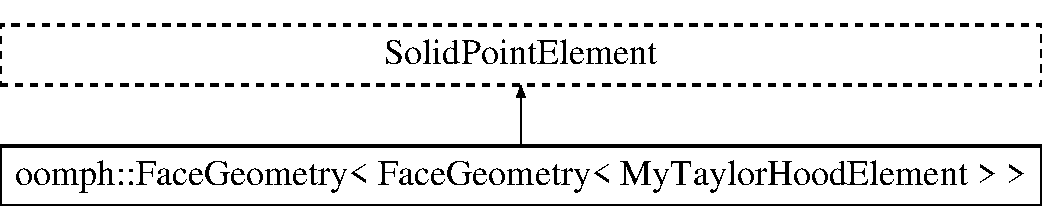
\includegraphics[height=2.000000cm]{classoomph_1_1FaceGeometry_3_01FaceGeometry_3_01MyTaylorHoodElement_01_4_01_4}
\end{center}
\end{figure}
\subsection*{Public Member Functions}
\begin{DoxyCompactItemize}
\item 
\hyperlink{classoomph_1_1FaceGeometry_3_01FaceGeometry_3_01MyTaylorHoodElement_01_4_01_4_a35f1bde1f3b3cc7c29d417cd75f0ef86}{Face\+Geometry} ()
\end{DoxyCompactItemize}


\subsection{Detailed Description}
\subsubsection*{template$<$$>$\newline
class oomph\+::\+Face\+Geometry$<$ Face\+Geometry$<$ My\+Taylor\+Hood\+Element $>$ $>$}

Face geometry for element is the same as that for the underlying wrapped element 

Definition at line 325 of file my\+\_\+taylor\+\_\+hood\+\_\+elements.\+h.



\subsection{Constructor \& Destructor Documentation}
\mbox{\Hypertarget{classoomph_1_1FaceGeometry_3_01FaceGeometry_3_01MyTaylorHoodElement_01_4_01_4_a35f1bde1f3b3cc7c29d417cd75f0ef86}\label{classoomph_1_1FaceGeometry_3_01FaceGeometry_3_01MyTaylorHoodElement_01_4_01_4_a35f1bde1f3b3cc7c29d417cd75f0ef86}} 
\index{oomph\+::\+Face\+Geometry$<$ Face\+Geometry$<$ My\+Taylor\+Hood\+Element $>$ $>$@{oomph\+::\+Face\+Geometry$<$ Face\+Geometry$<$ My\+Taylor\+Hood\+Element $>$ $>$}!Face\+Geometry@{Face\+Geometry}}
\index{Face\+Geometry@{Face\+Geometry}!oomph\+::\+Face\+Geometry$<$ Face\+Geometry$<$ My\+Taylor\+Hood\+Element $>$ $>$@{oomph\+::\+Face\+Geometry$<$ Face\+Geometry$<$ My\+Taylor\+Hood\+Element $>$ $>$}}
\subsubsection{\texorpdfstring{Face\+Geometry()}{FaceGeometry()}}
{\footnotesize\ttfamily oomph\+::\+Face\+Geometry$<$ Face\+Geometry$<$ \hyperlink{classoomph_1_1MyTaylorHoodElement}{My\+Taylor\+Hood\+Element} $>$ $>$\+::Face\+Geometry (\begin{DoxyParamCaption}{ }\end{DoxyParamCaption})\hspace{0.3cm}{\ttfamily [inline]}}



Definition at line 329 of file my\+\_\+taylor\+\_\+hood\+\_\+elements.\+h.



The documentation for this class was generated from the following file\+:\begin{DoxyCompactItemize}
\item 
\hyperlink{my__taylor__hood__elements_8h}{my\+\_\+taylor\+\_\+hood\+\_\+elements.\+h}\end{DoxyCompactItemize}

\hypertarget{classoomph_1_1FaceGeometry_3_01MyCrouzeixRaviartElement_01_4}{}\section{oomph\+:\+:Face\+Geometry$<$ My\+Crouzeix\+Raviart\+Element $>$ Class Template Reference}
\label{classoomph_1_1FaceGeometry_3_01MyCrouzeixRaviartElement_01_4}\index{oomph\+::\+Face\+Geometry$<$ My\+Crouzeix\+Raviart\+Element $>$@{oomph\+::\+Face\+Geometry$<$ My\+Crouzeix\+Raviart\+Element $>$}}
Inheritance diagram for oomph\+:\+:Face\+Geometry$<$ My\+Crouzeix\+Raviart\+Element $>$\+:\begin{figure}[H]
\begin{center}
\leavevmode
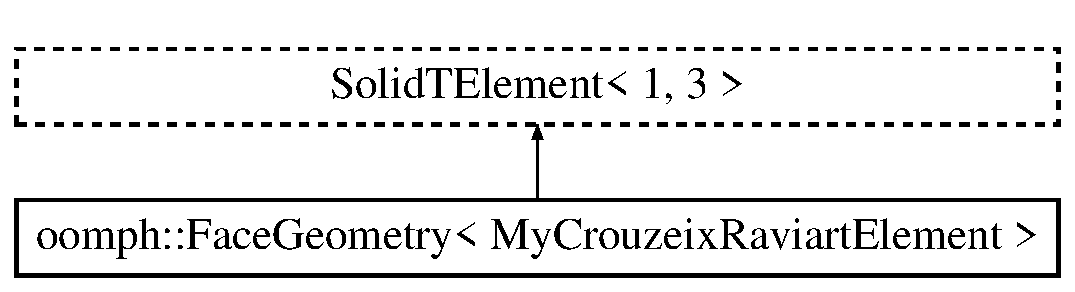
\includegraphics[height=2.000000cm]{classoomph_1_1FaceGeometry_3_01MyCrouzeixRaviartElement_01_4}
\end{center}
\end{figure}
\subsection*{Public Member Functions}
\begin{DoxyCompactItemize}
\item 
\hyperlink{classoomph_1_1FaceGeometry_3_01MyCrouzeixRaviartElement_01_4_a28b4b942614e6cfee40e773deb3e3003}{Face\+Geometry} ()
\end{DoxyCompactItemize}


\subsection{Detailed Description}
\subsubsection*{template$<$$>$\newline
class oomph\+::\+Face\+Geometry$<$ My\+Crouzeix\+Raviart\+Element $>$}

Face geometry for element is the same as that for the underlying wrapped element 

Definition at line 327 of file adaptive\+\_\+drop\+\_\+in\+\_\+channel.\+cc.



\subsection{Constructor \& Destructor Documentation}
\mbox{\Hypertarget{classoomph_1_1FaceGeometry_3_01MyCrouzeixRaviartElement_01_4_a28b4b942614e6cfee40e773deb3e3003}\label{classoomph_1_1FaceGeometry_3_01MyCrouzeixRaviartElement_01_4_a28b4b942614e6cfee40e773deb3e3003}} 
\index{oomph\+::\+Face\+Geometry$<$ My\+Crouzeix\+Raviart\+Element $>$@{oomph\+::\+Face\+Geometry$<$ My\+Crouzeix\+Raviart\+Element $>$}!Face\+Geometry@{Face\+Geometry}}
\index{Face\+Geometry@{Face\+Geometry}!oomph\+::\+Face\+Geometry$<$ My\+Crouzeix\+Raviart\+Element $>$@{oomph\+::\+Face\+Geometry$<$ My\+Crouzeix\+Raviart\+Element $>$}}
\subsubsection{\texorpdfstring{Face\+Geometry()}{FaceGeometry()}}
{\footnotesize\ttfamily oomph\+::\+Face\+Geometry$<$ \hyperlink{classoomph_1_1MyCrouzeixRaviartElement}{My\+Crouzeix\+Raviart\+Element} $>$\+::Face\+Geometry (\begin{DoxyParamCaption}{ }\end{DoxyParamCaption})\hspace{0.3cm}{\ttfamily [inline]}}



Definition at line 331 of file adaptive\+\_\+drop\+\_\+in\+\_\+channel.\+cc.



The documentation for this class was generated from the following file\+:\begin{DoxyCompactItemize}
\item 
\hyperlink{adaptive__drop__in__channel_8cc}{adaptive\+\_\+drop\+\_\+in\+\_\+channel.\+cc}\end{DoxyCompactItemize}

\hypertarget{classoomph_1_1FaceGeometry_3_01MyTaylorHoodElement_01_4}{}\section{oomph\+:\+:Face\+Geometry$<$ My\+Taylor\+Hood\+Element $>$ Class Template Reference}
\label{classoomph_1_1FaceGeometry_3_01MyTaylorHoodElement_01_4}\index{oomph\+::\+Face\+Geometry$<$ My\+Taylor\+Hood\+Element $>$@{oomph\+::\+Face\+Geometry$<$ My\+Taylor\+Hood\+Element $>$}}


{\ttfamily \#include $<$my\+\_\+taylor\+\_\+hood\+\_\+elements.\+h$>$}

Inheritance diagram for oomph\+:\+:Face\+Geometry$<$ My\+Taylor\+Hood\+Element $>$\+:\begin{figure}[H]
\begin{center}
\leavevmode
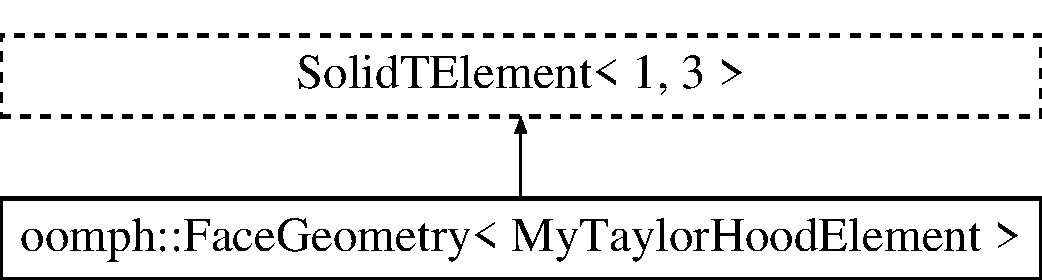
\includegraphics[height=2.000000cm]{classoomph_1_1FaceGeometry_3_01MyTaylorHoodElement_01_4}
\end{center}
\end{figure}
\subsection*{Public Member Functions}
\begin{DoxyCompactItemize}
\item 
\hyperlink{classoomph_1_1FaceGeometry_3_01MyTaylorHoodElement_01_4_a604dfaeec030bb7a08069c0e2c8805ab}{Face\+Geometry} ()
\end{DoxyCompactItemize}


\subsection{Detailed Description}
\subsubsection*{template$<$$>$\newline
class oomph\+::\+Face\+Geometry$<$ My\+Taylor\+Hood\+Element $>$}

Face geometry for element is the same as that for the underlying wrapped element 

Definition at line 313 of file my\+\_\+taylor\+\_\+hood\+\_\+elements.\+h.



\subsection{Constructor \& Destructor Documentation}
\mbox{\Hypertarget{classoomph_1_1FaceGeometry_3_01MyTaylorHoodElement_01_4_a604dfaeec030bb7a08069c0e2c8805ab}\label{classoomph_1_1FaceGeometry_3_01MyTaylorHoodElement_01_4_a604dfaeec030bb7a08069c0e2c8805ab}} 
\index{oomph\+::\+Face\+Geometry$<$ My\+Taylor\+Hood\+Element $>$@{oomph\+::\+Face\+Geometry$<$ My\+Taylor\+Hood\+Element $>$}!Face\+Geometry@{Face\+Geometry}}
\index{Face\+Geometry@{Face\+Geometry}!oomph\+::\+Face\+Geometry$<$ My\+Taylor\+Hood\+Element $>$@{oomph\+::\+Face\+Geometry$<$ My\+Taylor\+Hood\+Element $>$}}
\subsubsection{\texorpdfstring{Face\+Geometry()}{FaceGeometry()}}
{\footnotesize\ttfamily oomph\+::\+Face\+Geometry$<$ \hyperlink{classoomph_1_1MyTaylorHoodElement}{My\+Taylor\+Hood\+Element} $>$\+::Face\+Geometry (\begin{DoxyParamCaption}{ }\end{DoxyParamCaption})\hspace{0.3cm}{\ttfamily [inline]}}



Definition at line 317 of file my\+\_\+taylor\+\_\+hood\+\_\+elements.\+h.



The documentation for this class was generated from the following file\+:\begin{DoxyCompactItemize}
\item 
\hyperlink{my__taylor__hood__elements_8h}{my\+\_\+taylor\+\_\+hood\+\_\+elements.\+h}\end{DoxyCompactItemize}

\hypertarget{classoomph_1_1MyCrouzeixRaviartElement}{}\section{oomph\+:\+:My\+Crouzeix\+Raviart\+Element Class Reference}
\label{classoomph_1_1MyCrouzeixRaviartElement}\index{oomph\+::\+My\+Crouzeix\+Raviart\+Element@{oomph\+::\+My\+Crouzeix\+Raviart\+Element}}


Overload Crouzeix\+Raviart element to modify output.  


Inheritance diagram for oomph\+:\+:My\+Crouzeix\+Raviart\+Element\+:\begin{figure}[H]
\begin{center}
\leavevmode
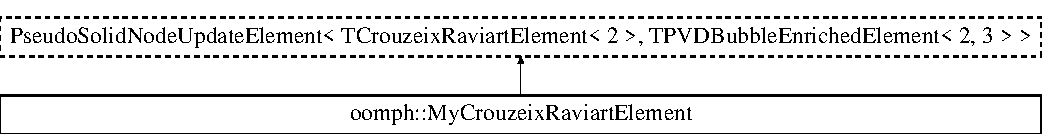
\includegraphics[height=1.800643cm]{classoomph_1_1MyCrouzeixRaviartElement}
\end{center}
\end{figure}
\subsection*{Public Member Functions}
\begin{DoxyCompactItemize}
\item 
\hyperlink{classoomph_1_1MyCrouzeixRaviartElement_a6719573c11157d360cb0a0fd0d2b92f4}{My\+Crouzeix\+Raviart\+Element} ()
\begin{DoxyCompactList}\small\item\em Constructor initialise error. \end{DoxyCompactList}\item 
void \hyperlink{classoomph_1_1MyCrouzeixRaviartElement_a0b1ccbfb0eda6807c3a332aa0b6ea6e2}{set\+\_\+error} (const double \&error)
\begin{DoxyCompactList}\small\item\em Set error value for post-\/processing. \end{DoxyCompactList}\item 
std\+::string \hyperlink{classoomph_1_1MyCrouzeixRaviartElement_afbec727a48f104b945cc54f798cbd1d3}{variable\+\_\+identifier} ()
\begin{DoxyCompactList}\small\item\em Return variable identifier. \end{DoxyCompactList}\item 
void \hyperlink{classoomph_1_1MyCrouzeixRaviartElement_ad1ea7115e6cb090d687ac421e56f4d16}{output} (std\+::ostream \&outfile, const unsigned \&nplot)
\begin{DoxyCompactList}\small\item\em Overload output function. \end{DoxyCompactList}\item 
double \hyperlink{classoomph_1_1MyCrouzeixRaviartElement_a18e8ab7199f42ca292214180ed86aa3a}{square\+\_\+of\+\_\+l2\+\_\+norm} ()
\begin{DoxyCompactList}\small\item\em Get square of L2 norm of velocity. \end{DoxyCompactList}\end{DoxyCompactItemize}
\subsection*{Private Attributes}
\begin{DoxyCompactItemize}
\item 
double \hyperlink{classoomph_1_1MyCrouzeixRaviartElement_aac525f961951f5d621f141b4fcdda357}{Error}
\begin{DoxyCompactList}\small\item\em Storage for elemental error estimate -- used for post-\/processing. \end{DoxyCompactList}\end{DoxyCompactItemize}


\subsection{Detailed Description}
Overload Crouzeix\+Raviart element to modify output. 

Definition at line 55 of file adaptive\+\_\+drop\+\_\+in\+\_\+channel.\+cc.



\subsection{Constructor \& Destructor Documentation}
\mbox{\Hypertarget{classoomph_1_1MyCrouzeixRaviartElement_a6719573c11157d360cb0a0fd0d2b92f4}\label{classoomph_1_1MyCrouzeixRaviartElement_a6719573c11157d360cb0a0fd0d2b92f4}} 
\index{oomph\+::\+My\+Crouzeix\+Raviart\+Element@{oomph\+::\+My\+Crouzeix\+Raviart\+Element}!My\+Crouzeix\+Raviart\+Element@{My\+Crouzeix\+Raviart\+Element}}
\index{My\+Crouzeix\+Raviart\+Element@{My\+Crouzeix\+Raviart\+Element}!oomph\+::\+My\+Crouzeix\+Raviart\+Element@{oomph\+::\+My\+Crouzeix\+Raviart\+Element}}
\subsubsection{\texorpdfstring{My\+Crouzeix\+Raviart\+Element()}{MyCrouzeixRaviartElement()}}
{\footnotesize\ttfamily oomph\+::\+My\+Crouzeix\+Raviart\+Element\+::\+My\+Crouzeix\+Raviart\+Element (\begin{DoxyParamCaption}{ }\end{DoxyParamCaption})\hspace{0.3cm}{\ttfamily [inline]}}



Constructor initialise error. 



Definition at line 68 of file adaptive\+\_\+drop\+\_\+in\+\_\+channel.\+cc.



\subsection{Member Function Documentation}
\mbox{\Hypertarget{classoomph_1_1MyCrouzeixRaviartElement_ad1ea7115e6cb090d687ac421e56f4d16}\label{classoomph_1_1MyCrouzeixRaviartElement_ad1ea7115e6cb090d687ac421e56f4d16}} 
\index{oomph\+::\+My\+Crouzeix\+Raviart\+Element@{oomph\+::\+My\+Crouzeix\+Raviart\+Element}!output@{output}}
\index{output@{output}!oomph\+::\+My\+Crouzeix\+Raviart\+Element@{oomph\+::\+My\+Crouzeix\+Raviart\+Element}}
\subsubsection{\texorpdfstring{output()}{output()}}
{\footnotesize\ttfamily void oomph\+::\+My\+Crouzeix\+Raviart\+Element\+::output (\begin{DoxyParamCaption}\item[{std\+::ostream \&}]{outfile,  }\item[{const unsigned \&}]{nplot }\end{DoxyParamCaption})\hspace{0.3cm}{\ttfamily [inline]}}



Overload output function. 



Definition at line 106 of file adaptive\+\_\+drop\+\_\+in\+\_\+channel.\+cc.

\mbox{\Hypertarget{classoomph_1_1MyCrouzeixRaviartElement_a0b1ccbfb0eda6807c3a332aa0b6ea6e2}\label{classoomph_1_1MyCrouzeixRaviartElement_a0b1ccbfb0eda6807c3a332aa0b6ea6e2}} 
\index{oomph\+::\+My\+Crouzeix\+Raviart\+Element@{oomph\+::\+My\+Crouzeix\+Raviart\+Element}!set\+\_\+error@{set\+\_\+error}}
\index{set\+\_\+error@{set\+\_\+error}!oomph\+::\+My\+Crouzeix\+Raviart\+Element@{oomph\+::\+My\+Crouzeix\+Raviart\+Element}}
\subsubsection{\texorpdfstring{set\+\_\+error()}{set\_error()}}
{\footnotesize\ttfamily void oomph\+::\+My\+Crouzeix\+Raviart\+Element\+::set\+\_\+error (\begin{DoxyParamCaption}\item[{const double \&}]{error }\end{DoxyParamCaption})\hspace{0.3cm}{\ttfamily [inline]}}



Set error value for post-\/processing. 



Definition at line 75 of file adaptive\+\_\+drop\+\_\+in\+\_\+channel.\+cc.

\mbox{\Hypertarget{classoomph_1_1MyCrouzeixRaviartElement_a18e8ab7199f42ca292214180ed86aa3a}\label{classoomph_1_1MyCrouzeixRaviartElement_a18e8ab7199f42ca292214180ed86aa3a}} 
\index{oomph\+::\+My\+Crouzeix\+Raviart\+Element@{oomph\+::\+My\+Crouzeix\+Raviart\+Element}!square\+\_\+of\+\_\+l2\+\_\+norm@{square\+\_\+of\+\_\+l2\+\_\+norm}}
\index{square\+\_\+of\+\_\+l2\+\_\+norm@{square\+\_\+of\+\_\+l2\+\_\+norm}!oomph\+::\+My\+Crouzeix\+Raviart\+Element@{oomph\+::\+My\+Crouzeix\+Raviart\+Element}}
\subsubsection{\texorpdfstring{square\+\_\+of\+\_\+l2\+\_\+norm()}{square\_of\_l2\_norm()}}
{\footnotesize\ttfamily double oomph\+::\+My\+Crouzeix\+Raviart\+Element\+::square\+\_\+of\+\_\+l2\+\_\+norm (\begin{DoxyParamCaption}{ }\end{DoxyParamCaption})\hspace{0.3cm}{\ttfamily [inline]}}



Get square of L2 norm of velocity. 



Definition at line 252 of file adaptive\+\_\+drop\+\_\+in\+\_\+channel.\+cc.

\mbox{\Hypertarget{classoomph_1_1MyCrouzeixRaviartElement_afbec727a48f104b945cc54f798cbd1d3}\label{classoomph_1_1MyCrouzeixRaviartElement_afbec727a48f104b945cc54f798cbd1d3}} 
\index{oomph\+::\+My\+Crouzeix\+Raviart\+Element@{oomph\+::\+My\+Crouzeix\+Raviart\+Element}!variable\+\_\+identifier@{variable\+\_\+identifier}}
\index{variable\+\_\+identifier@{variable\+\_\+identifier}!oomph\+::\+My\+Crouzeix\+Raviart\+Element@{oomph\+::\+My\+Crouzeix\+Raviart\+Element}}
\subsubsection{\texorpdfstring{variable\+\_\+identifier()}{variable\_identifier()}}
{\footnotesize\ttfamily std\+::string oomph\+::\+My\+Crouzeix\+Raviart\+Element\+::variable\+\_\+identifier (\begin{DoxyParamCaption}{ }\end{DoxyParamCaption})\hspace{0.3cm}{\ttfamily [inline]}}



Return variable identifier. 



Definition at line 78 of file adaptive\+\_\+drop\+\_\+in\+\_\+channel.\+cc.



\subsection{Member Data Documentation}
\mbox{\Hypertarget{classoomph_1_1MyCrouzeixRaviartElement_aac525f961951f5d621f141b4fcdda357}\label{classoomph_1_1MyCrouzeixRaviartElement_aac525f961951f5d621f141b4fcdda357}} 
\index{oomph\+::\+My\+Crouzeix\+Raviart\+Element@{oomph\+::\+My\+Crouzeix\+Raviart\+Element}!Error@{Error}}
\index{Error@{Error}!oomph\+::\+My\+Crouzeix\+Raviart\+Element@{oomph\+::\+My\+Crouzeix\+Raviart\+Element}}
\subsubsection{\texorpdfstring{Error}{Error}}
{\footnotesize\ttfamily double oomph\+::\+My\+Crouzeix\+Raviart\+Element\+::\+Error\hspace{0.3cm}{\ttfamily [private]}}



Storage for elemental error estimate -- used for post-\/processing. 



Definition at line 63 of file adaptive\+\_\+drop\+\_\+in\+\_\+channel.\+cc.



The documentation for this class was generated from the following file\+:\begin{DoxyCompactItemize}
\item 
\hyperlink{adaptive__drop__in__channel_8cc}{adaptive\+\_\+drop\+\_\+in\+\_\+channel.\+cc}\end{DoxyCompactItemize}

\hypertarget{classoomph_1_1MyTaylorHoodElement}{}\section{oomph\+:\+:My\+Taylor\+Hood\+Element Class Reference}
\label{classoomph_1_1MyTaylorHoodElement}\index{oomph\+::\+My\+Taylor\+Hood\+Element@{oomph\+::\+My\+Taylor\+Hood\+Element}}


Overload Taylor\+Hood element to modify output.  




{\ttfamily \#include $<$my\+\_\+taylor\+\_\+hood\+\_\+elements.\+h$>$}

Inheritance diagram for oomph\+:\+:My\+Taylor\+Hood\+Element\+:\begin{figure}[H]
\begin{center}
\leavevmode
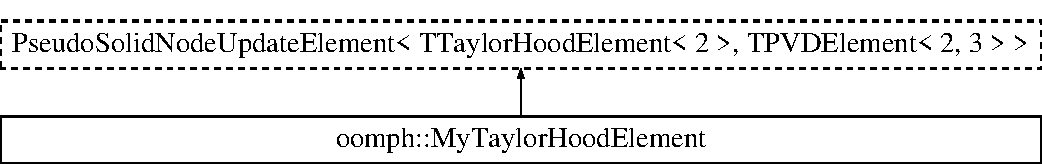
\includegraphics[height=2.000000cm]{classoomph_1_1MyTaylorHoodElement}
\end{center}
\end{figure}
\subsection*{Public Member Functions}
\begin{DoxyCompactItemize}
\item 
\hyperlink{classoomph_1_1MyTaylorHoodElement_a936bd6421ba42e5b73f983f5141b37c2}{My\+Taylor\+Hood\+Element} ()
\begin{DoxyCompactList}\small\item\em Constructor initialise error. \end{DoxyCompactList}\item 
void \hyperlink{classoomph_1_1MyTaylorHoodElement_ae4f6eea59b7bcf6e737d829b37c47fe9}{set\+\_\+error} (const double \&error)
\begin{DoxyCompactList}\small\item\em Set error value for post-\/processing. \end{DoxyCompactList}\item 
std\+::string \hyperlink{classoomph_1_1MyTaylorHoodElement_a429987090e76cd39a657b3a8eefbbbe9}{variable\+\_\+identifier} ()
\begin{DoxyCompactList}\small\item\em Return variable identifier. \end{DoxyCompactList}\item 
void \hyperlink{classoomph_1_1MyTaylorHoodElement_a5505717f2d16c2b231e7c347cb0c49b1}{output} (std\+::ostream \&outfile, const unsigned \&nplot)
\begin{DoxyCompactList}\small\item\em Overload output function. \end{DoxyCompactList}\item 
double \hyperlink{classoomph_1_1MyTaylorHoodElement_ad9efcab0ef22434e6fc5f2eb4b84643d}{square\+\_\+of\+\_\+l2\+\_\+norm} ()
\begin{DoxyCompactList}\small\item\em Get square of L2 norm of velocity. \end{DoxyCompactList}\end{DoxyCompactItemize}
\subsection*{Private Attributes}
\begin{DoxyCompactItemize}
\item 
double \hyperlink{classoomph_1_1MyTaylorHoodElement_a381cf2cdb628fb7aacfd6dd59dc2996b}{Error}
\begin{DoxyCompactList}\small\item\em Storage for elemental error estimate -- used for post-\/processing. \end{DoxyCompactList}\end{DoxyCompactItemize}


\subsection{Detailed Description}
Overload Taylor\+Hood element to modify output. 

Definition at line 39 of file my\+\_\+taylor\+\_\+hood\+\_\+elements.\+h.



\subsection{Constructor \& Destructor Documentation}
\mbox{\Hypertarget{classoomph_1_1MyTaylorHoodElement_a936bd6421ba42e5b73f983f5141b37c2}\label{classoomph_1_1MyTaylorHoodElement_a936bd6421ba42e5b73f983f5141b37c2}} 
\index{oomph\+::\+My\+Taylor\+Hood\+Element@{oomph\+::\+My\+Taylor\+Hood\+Element}!My\+Taylor\+Hood\+Element@{My\+Taylor\+Hood\+Element}}
\index{My\+Taylor\+Hood\+Element@{My\+Taylor\+Hood\+Element}!oomph\+::\+My\+Taylor\+Hood\+Element@{oomph\+::\+My\+Taylor\+Hood\+Element}}
\subsubsection{\texorpdfstring{My\+Taylor\+Hood\+Element()}{MyTaylorHoodElement()}}
{\footnotesize\ttfamily oomph\+::\+My\+Taylor\+Hood\+Element\+::\+My\+Taylor\+Hood\+Element (\begin{DoxyParamCaption}{ }\end{DoxyParamCaption})\hspace{0.3cm}{\ttfamily [inline]}}



Constructor initialise error. 



Definition at line 52 of file my\+\_\+taylor\+\_\+hood\+\_\+elements.\+h.



\subsection{Member Function Documentation}
\mbox{\Hypertarget{classoomph_1_1MyTaylorHoodElement_a5505717f2d16c2b231e7c347cb0c49b1}\label{classoomph_1_1MyTaylorHoodElement_a5505717f2d16c2b231e7c347cb0c49b1}} 
\index{oomph\+::\+My\+Taylor\+Hood\+Element@{oomph\+::\+My\+Taylor\+Hood\+Element}!output@{output}}
\index{output@{output}!oomph\+::\+My\+Taylor\+Hood\+Element@{oomph\+::\+My\+Taylor\+Hood\+Element}}
\subsubsection{\texorpdfstring{output()}{output()}}
{\footnotesize\ttfamily void oomph\+::\+My\+Taylor\+Hood\+Element\+::output (\begin{DoxyParamCaption}\item[{std\+::ostream \&}]{outfile,  }\item[{const unsigned \&}]{nplot }\end{DoxyParamCaption})\hspace{0.3cm}{\ttfamily [inline]}}



Overload output function. 



Definition at line 89 of file my\+\_\+taylor\+\_\+hood\+\_\+elements.\+h.

\mbox{\Hypertarget{classoomph_1_1MyTaylorHoodElement_ae4f6eea59b7bcf6e737d829b37c47fe9}\label{classoomph_1_1MyTaylorHoodElement_ae4f6eea59b7bcf6e737d829b37c47fe9}} 
\index{oomph\+::\+My\+Taylor\+Hood\+Element@{oomph\+::\+My\+Taylor\+Hood\+Element}!set\+\_\+error@{set\+\_\+error}}
\index{set\+\_\+error@{set\+\_\+error}!oomph\+::\+My\+Taylor\+Hood\+Element@{oomph\+::\+My\+Taylor\+Hood\+Element}}
\subsubsection{\texorpdfstring{set\+\_\+error()}{set\_error()}}
{\footnotesize\ttfamily void oomph\+::\+My\+Taylor\+Hood\+Element\+::set\+\_\+error (\begin{DoxyParamCaption}\item[{const double \&}]{error }\end{DoxyParamCaption})\hspace{0.3cm}{\ttfamily [inline]}}



Set error value for post-\/processing. 



Definition at line 58 of file my\+\_\+taylor\+\_\+hood\+\_\+elements.\+h.

\mbox{\Hypertarget{classoomph_1_1MyTaylorHoodElement_ad9efcab0ef22434e6fc5f2eb4b84643d}\label{classoomph_1_1MyTaylorHoodElement_ad9efcab0ef22434e6fc5f2eb4b84643d}} 
\index{oomph\+::\+My\+Taylor\+Hood\+Element@{oomph\+::\+My\+Taylor\+Hood\+Element}!square\+\_\+of\+\_\+l2\+\_\+norm@{square\+\_\+of\+\_\+l2\+\_\+norm}}
\index{square\+\_\+of\+\_\+l2\+\_\+norm@{square\+\_\+of\+\_\+l2\+\_\+norm}!oomph\+::\+My\+Taylor\+Hood\+Element@{oomph\+::\+My\+Taylor\+Hood\+Element}}
\subsubsection{\texorpdfstring{square\+\_\+of\+\_\+l2\+\_\+norm()}{square\_of\_l2\_norm()}}
{\footnotesize\ttfamily double oomph\+::\+My\+Taylor\+Hood\+Element\+::square\+\_\+of\+\_\+l2\+\_\+norm (\begin{DoxyParamCaption}{ }\end{DoxyParamCaption})\hspace{0.3cm}{\ttfamily [inline]}}



Get square of L2 norm of velocity. 



Definition at line 235 of file my\+\_\+taylor\+\_\+hood\+\_\+elements.\+h.

\mbox{\Hypertarget{classoomph_1_1MyTaylorHoodElement_a429987090e76cd39a657b3a8eefbbbe9}\label{classoomph_1_1MyTaylorHoodElement_a429987090e76cd39a657b3a8eefbbbe9}} 
\index{oomph\+::\+My\+Taylor\+Hood\+Element@{oomph\+::\+My\+Taylor\+Hood\+Element}!variable\+\_\+identifier@{variable\+\_\+identifier}}
\index{variable\+\_\+identifier@{variable\+\_\+identifier}!oomph\+::\+My\+Taylor\+Hood\+Element@{oomph\+::\+My\+Taylor\+Hood\+Element}}
\subsubsection{\texorpdfstring{variable\+\_\+identifier()}{variable\_identifier()}}
{\footnotesize\ttfamily std\+::string oomph\+::\+My\+Taylor\+Hood\+Element\+::variable\+\_\+identifier (\begin{DoxyParamCaption}{ }\end{DoxyParamCaption})\hspace{0.3cm}{\ttfamily [inline]}}



Return variable identifier. 



Definition at line 61 of file my\+\_\+taylor\+\_\+hood\+\_\+elements.\+h.



\subsection{Member Data Documentation}
\mbox{\Hypertarget{classoomph_1_1MyTaylorHoodElement_a381cf2cdb628fb7aacfd6dd59dc2996b}\label{classoomph_1_1MyTaylorHoodElement_a381cf2cdb628fb7aacfd6dd59dc2996b}} 
\index{oomph\+::\+My\+Taylor\+Hood\+Element@{oomph\+::\+My\+Taylor\+Hood\+Element}!Error@{Error}}
\index{Error@{Error}!oomph\+::\+My\+Taylor\+Hood\+Element@{oomph\+::\+My\+Taylor\+Hood\+Element}}
\subsubsection{\texorpdfstring{Error}{Error}}
{\footnotesize\ttfamily double oomph\+::\+My\+Taylor\+Hood\+Element\+::\+Error\hspace{0.3cm}{\ttfamily [private]}}



Storage for elemental error estimate -- used for post-\/processing. 



Definition at line 47 of file my\+\_\+taylor\+\_\+hood\+\_\+elements.\+h.



The documentation for this class was generated from the following file\+:\begin{DoxyCompactItemize}
\item 
\hyperlink{my__taylor__hood__elements_8h}{my\+\_\+taylor\+\_\+hood\+\_\+elements.\+h}\end{DoxyCompactItemize}

\chapter{File Documentation}
\hypertarget{adaptive__bubble__in__channel_8cc}{}\section{adaptive\+\_\+bubble\+\_\+in\+\_\+channel.\+cc File Reference}
\label{adaptive__bubble__in__channel_8cc}\index{adaptive\+\_\+bubble\+\_\+in\+\_\+channel.\+cc@{adaptive\+\_\+bubble\+\_\+in\+\_\+channel.\+cc}}
\subsection*{Classes}
\begin{DoxyCompactItemize}
\item 
class \hyperlink{classoomph_1_1MyTaylorHoodElement}{oomph\+::\+My\+Taylor\+Hood\+Element}
\begin{DoxyCompactList}\small\item\em Overload Taylor\+Hood element to modify output. \end{DoxyCompactList}\item 
class \hyperlink{classoomph_1_1FaceGeometry_3_01MyTaylorHoodElement_01_4}{oomph\+::\+Face\+Geometry$<$ My\+Taylor\+Hood\+Element $>$}
\item 
class \hyperlink{classoomph_1_1FaceGeometry_3_01FaceGeometry_3_01MyTaylorHoodElement_01_4_01_4}{oomph\+::\+Face\+Geometry$<$ Face\+Geometry$<$ My\+Taylor\+Hood\+Element $>$ $>$}
\item 
class \hyperlink{classBubbleInChannelProblem}{Bubble\+In\+Channel\+Problem$<$ E\+L\+E\+M\+E\+N\+T $>$}
\begin{DoxyCompactList}\small\item\em Problem class to simulate inviscid bubble propagating along 2D channel. \end{DoxyCompactList}\end{DoxyCompactItemize}
\subsection*{Namespaces}
\begin{DoxyCompactItemize}
\item 
 \hyperlink{namespaceoomph}{oomph}
\item 
 \hyperlink{namespaceProblem__Parameter}{Problem\+\_\+\+Parameter}
\begin{DoxyCompactList}\small\item\em Namespace for Problem Parameter. \end{DoxyCompactList}\end{DoxyCompactItemize}
\subsection*{Functions}
\begin{DoxyCompactItemize}
\item 
int \hyperlink{adaptive__bubble__in__channel_8cc_a3c04138a5bfe5d72780bb7e82a18e627}{main} (int argc, char $\ast$$\ast$argv)
\begin{DoxyCompactList}\small\item\em Driver code for moving bubble problem. \end{DoxyCompactList}\end{DoxyCompactItemize}
\subsection*{Variables}
\begin{DoxyCompactItemize}
\item 
Doc\+Info \hyperlink{namespaceProblem__Parameter_a1dd3c6bcf97360c8fe0d288ca7610351}{Problem\+\_\+\+Parameter\+::\+Doc\+\_\+info}
\begin{DoxyCompactList}\small\item\em Doc info object. \end{DoxyCompactList}\item 
double \hyperlink{namespaceProblem__Parameter_acc656299287d4d9a8374c2c501750b4f}{Problem\+\_\+\+Parameter\+::\+Re} =0.\+0
\begin{DoxyCompactList}\small\item\em Reynolds number. \end{DoxyCompactList}\item 
double \hyperlink{namespaceProblem__Parameter_af6194d2571881779c678fbabc1503d47}{Problem\+\_\+\+Parameter\+::\+Ca} = 10.\+0
\begin{DoxyCompactList}\small\item\em Capillary number. \end{DoxyCompactList}\item 
double \hyperlink{namespaceProblem__Parameter_abec2e733c8f2d3c18ebc702b3f80cc17}{Problem\+\_\+\+Parameter\+::\+Nu} =0.\+3
\begin{DoxyCompactList}\small\item\em Pseudo-\/solid Poisson ratio. \end{DoxyCompactList}\item 
double \hyperlink{namespaceProblem__Parameter_a903237528f0e9bb92debcc8842576cca}{Problem\+\_\+\+Parameter\+::\+Radius} = 0.\+25
\begin{DoxyCompactList}\small\item\em Initial radius of bubble. \end{DoxyCompactList}\item 
double \hyperlink{namespaceProblem__Parameter_aad8e0a2d1ec39a8dd7357a43bcc5f20e}{Problem\+\_\+\+Parameter\+::\+Volume} = -\/Mathematical\+Constants\+::\+Pi$\ast$Radius$\ast$Radius
\begin{DoxyCompactList}\small\item\em Volume of the bubble (negative because it\textquotesingle{}s outside the fluid!) \end{DoxyCompactList}\item 
double \hyperlink{namespaceProblem__Parameter_a7792613e563a733ad88b8e15d126fc3a}{Problem\+\_\+\+Parameter\+::\+Inflow\+\_\+veloc\+\_\+magnitude} = 0.\+0
\begin{DoxyCompactList}\small\item\em Scaling factor for inflow velocity (allows it to be switched off to do hydrostatics) \end{DoxyCompactList}\item 
double \hyperlink{namespaceProblem__Parameter_a7b67840fea463f29b53d12f7bd7cb34b}{Problem\+\_\+\+Parameter\+::\+Length} = 3.\+0
\begin{DoxyCompactList}\small\item\em Length of the channel. \end{DoxyCompactList}\item 
Constitutive\+Law $\ast$ \hyperlink{namespaceProblem__Parameter_a810f05c8d3e3331aed75643557d1057c}{Problem\+\_\+\+Parameter\+::\+Constitutive\+\_\+law\+\_\+pt} =0
\begin{DoxyCompactList}\small\item\em Constitutive law used to determine the mesh deformation. \end{DoxyCompactList}\item 
ofstream \hyperlink{namespaceProblem__Parameter_a55310be5f2dfcb5fcfe35d71f9c16e06}{Problem\+\_\+\+Parameter\+::\+Trace\+\_\+file}
\begin{DoxyCompactList}\small\item\em Trace file. \end{DoxyCompactList}\item 
ofstream \hyperlink{namespaceProblem__Parameter_a388e06a5e637b21378ab1832e5564bec}{Problem\+\_\+\+Parameter\+::\+Norm\+\_\+file}
\begin{DoxyCompactList}\small\item\em File to document the norm of the solution (for validation purposes -- triangle doesn\textquotesingle{}t give fully reproducible results so mesh generation/adaptation may generate slightly different numbers of elements on different machines!) \end{DoxyCompactList}\end{DoxyCompactItemize}


\subsection{Function Documentation}
\mbox{\Hypertarget{adaptive__bubble__in__channel_8cc_a3c04138a5bfe5d72780bb7e82a18e627}\label{adaptive__bubble__in__channel_8cc_a3c04138a5bfe5d72780bb7e82a18e627}} 
\index{adaptive\+\_\+bubble\+\_\+in\+\_\+channel.\+cc@{adaptive\+\_\+bubble\+\_\+in\+\_\+channel.\+cc}!main@{main}}
\index{main@{main}!adaptive\+\_\+bubble\+\_\+in\+\_\+channel.\+cc@{adaptive\+\_\+bubble\+\_\+in\+\_\+channel.\+cc}}
\subsubsection{\texorpdfstring{main()}{main()}}
{\footnotesize\ttfamily int main (\begin{DoxyParamCaption}\item[{int}]{argc,  }\item[{char $\ast$$\ast$}]{argv }\end{DoxyParamCaption})}



Driver code for moving bubble problem. 



Definition at line 1276 of file adaptive\+\_\+bubble\+\_\+in\+\_\+channel.\+cc.



References Bubble\+In\+Channel\+Problem$<$ E\+L\+E\+M\+E\+N\+T $>$\+::complete\+\_\+problem\+\_\+setup(), Problem\+\_\+\+Parameter\+::\+Constitutive\+\_\+law\+\_\+pt, Bubble\+In\+Channel\+Problem$<$ E\+L\+E\+M\+E\+N\+T $>$\+::doc\+\_\+solution(), Problem\+\_\+\+Parameter\+::\+Inflow\+\_\+veloc\+\_\+magnitude, Problem\+\_\+\+Parameter\+::\+Norm\+\_\+file, Problem\+\_\+\+Parameter\+::\+Nu, and Problem\+\_\+\+Parameter\+::\+Trace\+\_\+file.


\hypertarget{adaptive__bubble__in__channel_8txt__doxygenified_8h}{}\section{adaptive\+\_\+bubble\+\_\+in\+\_\+channel.\+txt\+\_\+doxygenified.\+h File Reference}
\label{adaptive__bubble__in__channel_8txt__doxygenified_8h}\index{adaptive\+\_\+bubble\+\_\+in\+\_\+channel.\+txt\+\_\+doxygenified.\+h@{adaptive\+\_\+bubble\+\_\+in\+\_\+channel.\+txt\+\_\+doxygenified.\+h}}

\hypertarget{adaptive__drop__in__channel_8cc}{}\section{adaptive\+\_\+drop\+\_\+in\+\_\+channel.\+cc File Reference}
\label{adaptive__drop__in__channel_8cc}\index{adaptive\+\_\+drop\+\_\+in\+\_\+channel.\+cc@{adaptive\+\_\+drop\+\_\+in\+\_\+channel.\+cc}}
\subsection*{Classes}
\begin{DoxyCompactItemize}
\item 
class \hyperlink{classoomph_1_1MyCrouzeixRaviartElement}{oomph\+::\+My\+Crouzeix\+Raviart\+Element}
\begin{DoxyCompactList}\small\item\em Overload Crouzeix\+Raviart element to modify output. \end{DoxyCompactList}\item 
class \hyperlink{classoomph_1_1FaceGeometry_3_01MyCrouzeixRaviartElement_01_4}{oomph\+::\+Face\+Geometry$<$ My\+Crouzeix\+Raviart\+Element $>$}
\item 
class \hyperlink{classoomph_1_1FaceGeometry_3_01FaceGeometry_3_01MyCrouzeixRaviartElement_01_4_01_4}{oomph\+::\+Face\+Geometry$<$ Face\+Geometry$<$ My\+Crouzeix\+Raviart\+Element $>$ $>$}
\item 
class \hyperlink{classDropInChannelProblem}{Drop\+In\+Channel\+Problem$<$ E\+L\+E\+M\+E\+N\+T $>$}
\begin{DoxyCompactList}\small\item\em Problem class to simulate viscous drop propagating along 2D channel. \end{DoxyCompactList}\end{DoxyCompactItemize}
\subsection*{Namespaces}
\begin{DoxyCompactItemize}
\item 
 \hyperlink{namespaceoomph}{oomph}
\item 
 \hyperlink{namespaceProblem__Parameter}{Problem\+\_\+\+Parameter}
\begin{DoxyCompactList}\small\item\em Namespace for Problem Parameter. \end{DoxyCompactList}\end{DoxyCompactItemize}
\subsection*{Functions}
\begin{DoxyCompactItemize}
\item 
int \hyperlink{adaptive__drop__in__channel_8cc_a3c04138a5bfe5d72780bb7e82a18e627}{main} (int argc, char $\ast$$\ast$argv)
\begin{DoxyCompactList}\small\item\em Driver code for moving block problem. \end{DoxyCompactList}\end{DoxyCompactItemize}
\subsection*{Variables}
\begin{DoxyCompactItemize}
\item 
double \hyperlink{namespaceProblem__Parameter_afdb95f68bd3c77e4c12001a29bd26e31}{Problem\+\_\+\+Parameter\+::\+Viscosity\+\_\+ratio} = 10.\+0
\begin{DoxyCompactList}\small\item\em Viscosity ratio of the droplet to the surrounding fluid. \end{DoxyCompactList}\end{DoxyCompactItemize}


\subsection{Function Documentation}
\mbox{\Hypertarget{adaptive__drop__in__channel_8cc_a3c04138a5bfe5d72780bb7e82a18e627}\label{adaptive__drop__in__channel_8cc_a3c04138a5bfe5d72780bb7e82a18e627}} 
\index{adaptive\+\_\+drop\+\_\+in\+\_\+channel.\+cc@{adaptive\+\_\+drop\+\_\+in\+\_\+channel.\+cc}!main@{main}}
\index{main@{main}!adaptive\+\_\+drop\+\_\+in\+\_\+channel.\+cc@{adaptive\+\_\+drop\+\_\+in\+\_\+channel.\+cc}}
\subsubsection{\texorpdfstring{main()}{main()}}
{\footnotesize\ttfamily int main (\begin{DoxyParamCaption}\item[{int}]{argc,  }\item[{char $\ast$$\ast$}]{argv }\end{DoxyParamCaption})}



Driver code for moving block problem. 



Definition at line 1307 of file adaptive\+\_\+drop\+\_\+in\+\_\+channel.\+cc.



References Problem\+\_\+\+Parameter\+::\+Ca, Problem\+\_\+\+Parameter\+::\+Constitutive\+\_\+law\+\_\+pt, Problem\+\_\+\+Parameter\+::\+Inflow\+\_\+veloc\+\_\+magnitude, Problem\+\_\+\+Parameter\+::\+Norm\+\_\+file, Problem\+\_\+\+Parameter\+::\+Nu, and Problem\+\_\+\+Parameter\+::\+Trace\+\_\+file.


%--- End generated contents ---

% Index
\backmatter
\newpage
\phantomsection
\clearemptydoublepage
\addcontentsline{toc}{chapter}{Index}
\printindex

